\documentclass[a4paper,english,titlepage,12pt]{article} 
\usepackage[english]{babel}
\usepackage[table]{xcolor}

% Some default packages
\usepackage[utf8]{inputenc}
\usepackage[T1]{fontenc}  % Should help with special characters
\usepackage{ifpdf}        % PDF check
\usepackage{fancyhdr}	  % Page number on top
\usepackage{parskip}	  % Change paragraphs with space not indent
\usepackage{pdfpages}	 % Attach PDF documents
\usepackage{setspace}	 % Control line space
\usepackage{graphicx}	 % Graphics
\usepackage{float}	     % Graphics layout
\usepackage{caption}
\usepackage{geometry}

% Neutral links
\usepackage[pdfpagemode=None, colorlinks=true, urlcolor=blue, linkcolor=black, citecolor=black, pdfstartview=FitH]{hyperref}

% Math packages
\usepackage{amsmath}
\usepackage{amssymb}
\usepackage{latexsym}

% Source code
%\usepackage{listings}

% Sub figures
%\usepackage{subfig}
\usepackage{subcaption}
\usepackage{graphicx}

% Algorithm pseudo code
\usepackage{algorithm}
\usepackage{algorithmic}

% Natural references, e.g. Name [2001], [Name 1992]
\usepackage[square,numbers]{natbib}

% To-do comments
\usepackage[colorinlistoftodos]{todonotes}

% Table settings
% \setlength{\arrayrulewidth}{1mm}
% \setlength{\tabcolsep}{18pt}
\renewcommand{\arraystretch}{1.5}

% Inline comment
\newcommand{\todoinline}{\todo[inline,color=green!40]}

% Vectors, transposes, norms, absolutes, floor made easy
\newcommand{\vect}[1]{\ensuremath{\mathbf{#1}}}
\newcommand{\trans}[1]{\ensuremath\vect{#1}^\top}
\newcommand{\norm}[1]{\ensuremath\Vert #1 \Vert}
\newcommand{\abs}[1]{\ensuremath|#1|}
\newcommand{\floor}[1]{\ensuremath\lfloor#1\rfloor}

% Domains of real and natural numbers
\newcommand{\R}{\ensuremath\mathbb{R}}
\newcommand{\N}{\ensuremath\mathbb{N}}

\begin{document}

\ifpdf
\DeclareGraphicsExtensions{.pdf, .jpg, .tif}
\else
\DeclareGraphicsExtensions{.eps, .jpg}
\fi

% Page numbering begins with roman numbers (titlepage parameter removes page number from first page)
\pagenumbering{roman}
\pagestyle{empty} % Hides page numbers from beginning

\begin{titlepage}
	Aalto University \\
	School of Science \\
	Degree programme in Engineering Physics and Mathematics \\
	
	\vfill
	
	\begin{center}
		\begin{spacing}{1.75}
		{\LARGE Comparison of line search methods in unconstrained optimization}
		\end{spacing}
		
		Bachelor's Thesis \\
	    1.5.2019

		\vspace{3cm}

		{\large Einari Tuukkanen}

	\end{center}

	\vfill

	% Licensing
	The document can be stored and made available to the public on the open internet pages of Aalto University. \\\\
	All other rights are reserved.
\end{titlepage}

% TIIVISTELMÄPOHJA
%  Lataa tiivistelmäpohja täytettäväksi osoitteesta
%  https://noppa.aalto.fi/noppa/kurssi/tfm.kand/materiaali
%  ja tallenna se PDF-muodossa nimellä tiivistelma.pdf tähän hakemistoon
%
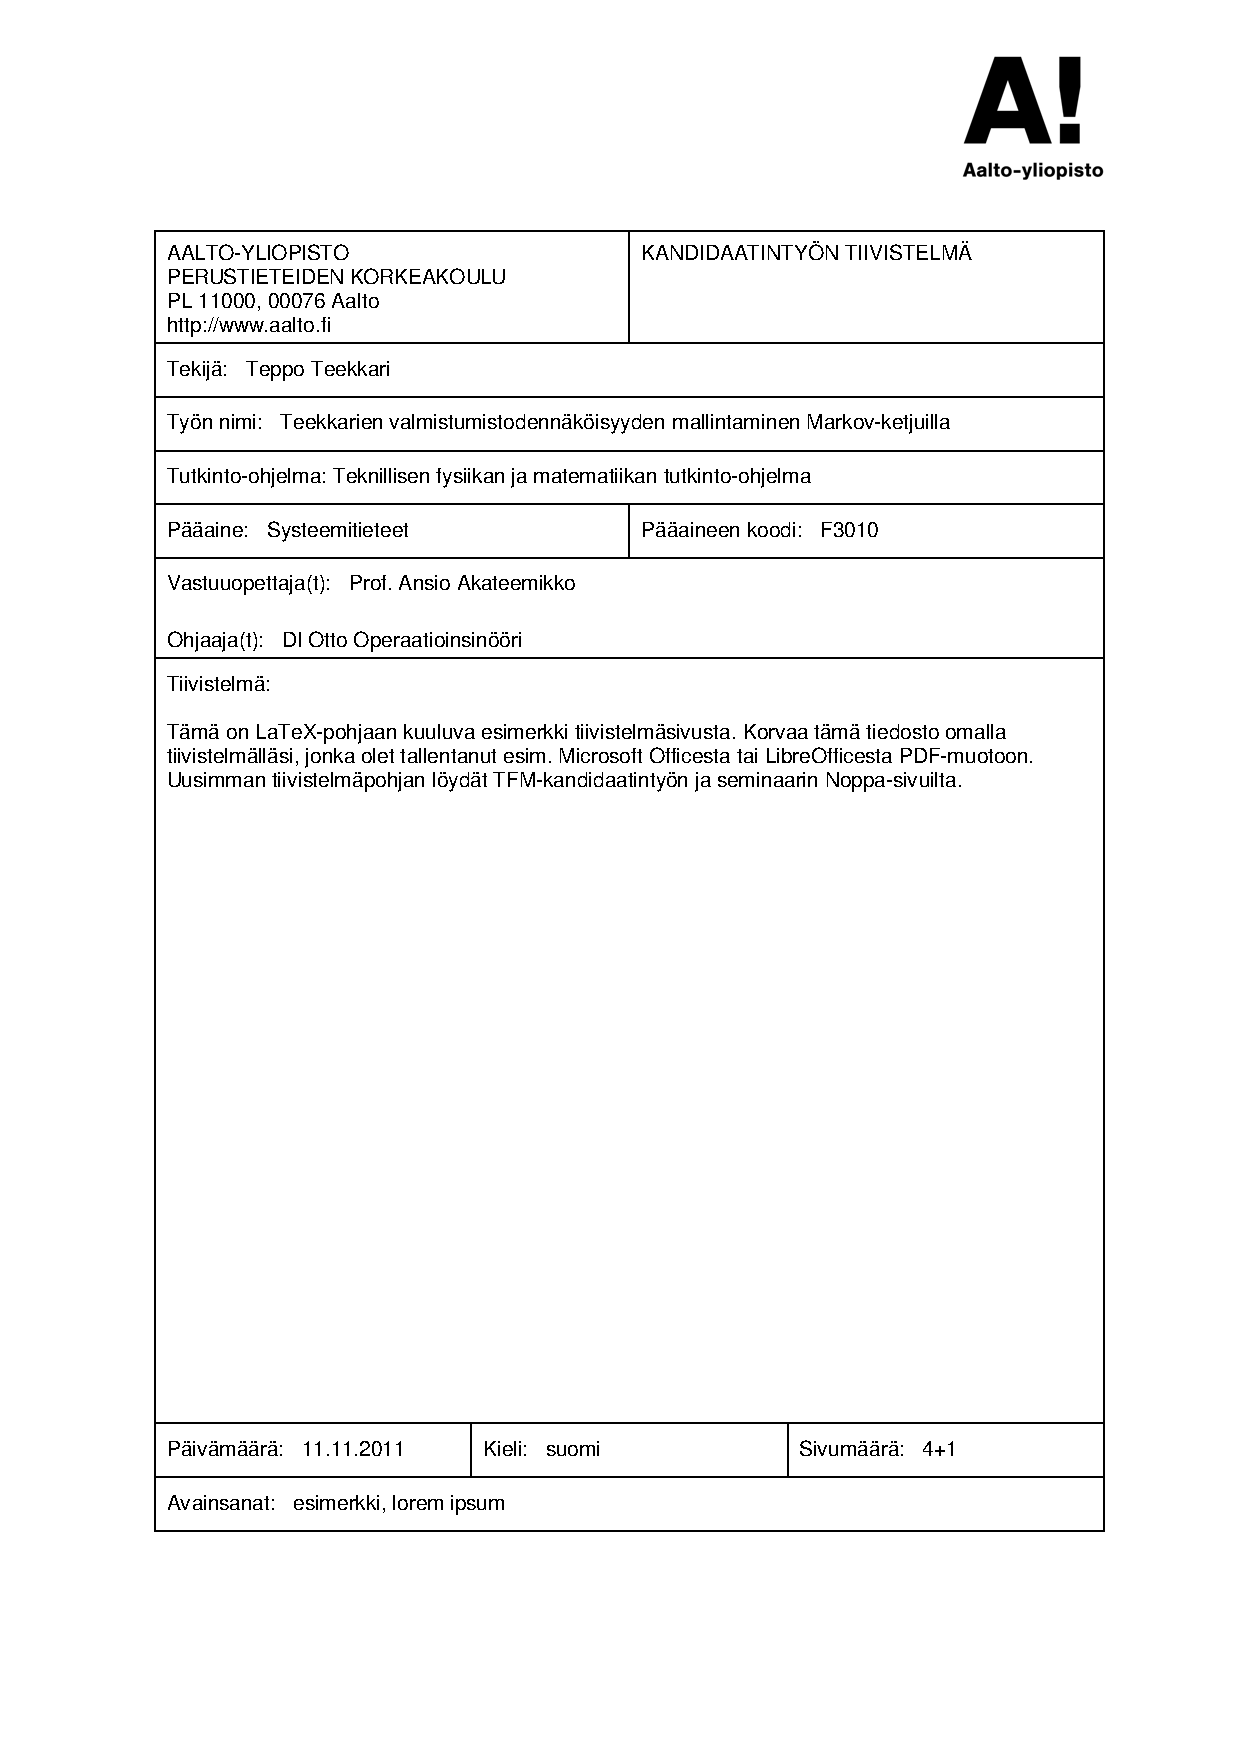
\includepdf{tiivistelma}

% Sisällysluettelo
\tableofcontents
\newpage

% Aloita todellinen sivunumerointi ensimmäisestä sisältösivusta
\pagestyle{fancy}

% Tyhjennetään kentät ja muotoilu
\fancyhf{}
\renewcommand{\headrulewidth}{0pt}
\renewcommand{\footrulewidth}{0pt}

% Sivunnumero ylhäällä oikealla
\rhead{\footnotesize \thepage} 
\pagenumbering{arabic}

% Ensimmäisellä sivulla ei kuitenkaan näytetä numeroa
\thispagestyle{empty} 


\section{Introduction}

Unconstrained nonlinear optimization has numerous real-life applications in different fields of science and technology such as in computational biology, machine learning, and finance.
In general, an unconstrained optimization problem can be formulated as
\begin{equation}\label{eq:minfx}
    \mathrm{min}_{\vect{x} \in \R^n} f(\vect{x}),
\end{equation}

where $f : \R^n \rightarrow \R$ is called an \emph{objective function} (or a \emph{target function}), and we are looking for a \emph{solution} vector $\vect{x}^* \in \R^n$ that minimizes the value of $f$ such that $f(\vect{x}^*) \leq f(\vect{x})$ for all $\vect{x}\in \R^n$. There are several different optimization algorithms (or methods) that can be used to solve the problem \eqref{eq:minfx}, e.g., Newton's and Conjugate Gradient methods \cite{book:nonlinear_programming}. However, the performances of different optimization methods typically vary significantly for different objective functions $f$, and it can be difficult to find the best solution method for a given problem instance. For example, we may use a different method when $f$ is convex compared to when $f$ is non-convex and has multiple local optima. Moreover, some methods are feasible only when $f$ satisfies certain properties, such as being continuously differentiable up to $n$ times.

While there are countless real-life problems that satisfy these conditions, they are often extremely complex and finding a global minimizing solution can be difficult.
Therefore, artificial problems are often used instead in developing and benchmarking optimization algorithms. \cite{test_function_collection_artifical}

In general, optimization algorithms are iterative processes that harness the processing power of computers efficiently by exploiting the properties of the target function $f$ in order for it to converge to an optimal solution.

The commonly used optimization methods typically start from a given point, choose a direction and a step size, and move to a new point. Then, different stopping criteria can be used to check if a minimizing solution has been found, and if not, the process is repeated until a minimum solution is reached or some other condition, such as maximum time limit or iteration count, is exceeded.

The step size is often computed by a separate \emph{line search} algorithm. After computing the target function value $f(\vect{x}')$ at a given point $\vect{x}'\in \R$, and a new direction $\vect{d}\in \R^n$, the line search function takes the form $f(\vect{x}' + \lambda \vect{d})$ which is a one-dimensional function of the step size $\lambda\in \R$. Line search algorithms try to find the value of $\lambda$ that minimizes this function, i.e., they try to solve the problem
\begin{equation}\label{eq:ls}
\mathop{\text{argmin}}_{\lambda\in \R} f(\vect{x}' + \lambda \vect{d})
\end{equation}
either approximately or exactly. Thus, line search algorithms are basically univariate optimization methods. Similarly to the multidimensional optimization methods, there are a number of different algorithms for finding the optimal step size, the simplest being just using a constant step size $\lambda$ for every iteration. 

In this thesis, we will investigate the effects of different line search algorithms on the overall performance of different optimization methods. The optimization methods investigated are mostly based on the algorithms represented in the Nonlinear Optimization course that was lectured in Fall 2018 and 2019 in Aalto University.

The main goal of this thesis is to investigate how different line search algorithms affect the performance of optimization methods for unconstrained nonlinear optimization problems on a general level. In addition, we will analyze the performance differences caused by the different line search methods with the goal of finding metrics that give us the best overall view of the algorithm's performance.

\subsection{Organization of this thesis}

\subsection*{Abbreviations and symbols used}

\begin{table}[H]
  \captionof{table}{Abbreviations used in this thesis, and their explanations.}
  \label{tab:abbreviations}
  \centering
  \rowcolors{2}{white}{gray!5}
  \begin{tabular}{|l|l|}
  \hline
  \rowcolor{gray!25}
  \textbf{Abbreviation} & \textbf{Explanation} \\
  \hline
  MM                    & main method, an unconstrained optimization method                               \\
  LS                    & line search, provides step sizes for main methods                               \\
  NM                    & Newton's Method                                                                 \\
  GDM                   & Gradient Descent Method                                                         \\
  CGM                   & Conjugate Gradient Method                                                       \\
  HBM                   & Heavy Ball Method                                                               \\
  CS                    & Constant search i.e. constant step size                                         \\
  GSS                   & Golden Section line search                                                      \\
  BS                    & Bisection line search                                                           \\
  DS                    & Dichotomous line search                                                         \\
  FS                    & Fibonacci line search                                                           \\
  US                    & Uniform line search                                                             \\
  NS                    & Newton's line search                                                            \\
  AS                    & Armijo's line search                                                            \\
  MSS                   & Matrix Square Sum target function                                               \\
  NE                    & Negative Entropy target function                                                \\
  \hline
  \end{tabular}
\end{table}


\section{Theory}


\subsection{Target Functions}


\subsubsection{Choosing target functions}


One of the biggest factors affecting the performance of an optimization algorithm is the target function of the problem we are solving. 
In this thesis we are going to examine two different problems with convex and differentiable target functions $f : \R^n \rightarrow \R$ of dimension $n = 50$. 

\subsubsection{Step size function}

Each optimization method involves computing a step at each iteration which is an optimization problem of the form \eqref{eq:ls}. In practice, at iteration $k$ we are at a point $\vect{x}^k$ and have computed the new direction vector $\vect{d}^k$. To simplify notation, we can define a step size function $g_{\vect{x}^k, \vect{d}^k}(\lambda) = f(\vect{x}^k + \lambda \vect{d}^k)$ for each of the target functions. Then at each iteration $k$ of the main optimization method, a new step size function is generated with the updated point $\vect{x}^k$ and direction vector $\vect{d}^k$.

\subsubsection{Matrix Square Sum}
\label{sect:matrix_square_sum}

The Matrix Square Sum is an extension to the Sum of Squares Function, which is defined as
\begin{equation}
    f(\mathbf{x})=f(x_1, ..., x_n)=\sum_{i=1}^{n}{ix_i^2}.
\end{equation}

To make Sum of Squares problem more difficult to solve, we are going modify it by adding three constants $A$, $b$ and $c$. Together they form what we are going to call a Matrix Square Sum function, defined as
\begin{equation}
    f(\vect{x}) = \norm{A \vect{x} + \vect{b}} ^ 2 + c \norm{\vect{x}} ^ 2,
\end{equation}

where $A$ is a positive definite (PD) $n \times n$ matrix, $\vect{x}$ and $\vect{b}$ are vectors of length $n$, and the scalar $c$ is a positive constant.

While $A$ could in theory be any $m \times n$ matrix, we are limiting it to be a PD square matrix to ensure that the function is strictly convex and has a unique global minimum. The matrix $A$ is formed in a few steps by first generating an initial $n \times n$ matrix $A'$ with random values $a_{ij} \in [-0.5, 0.5]\ \forall\ i,j = 1 \dots n$. Then we attempt to transform $A$ into a PD-matrix by $A = 0.5 (A' + A'^\top)$. Finally, if  $A$ is still not PD, it is modified by the formula 
\begin{equation}
    A = A + (\abs{\lambda_{min}} + d) I,
\end{equation}
where $\lambda_{min}$ is the minimum eigenvalue of $A$ and $d$ is a constant. The value of $d$ also determines $A$'s condition number defined as $\frac{\lambda_{max}}{\lambda_{min}}$ \cite{book:numberical_linear_algebra}. Smaller values of $d$ make the function more elliptic and harder for gradient methods to solve, while larger values produce higher condition numbers and more circular gradient curves, which makes the problem easier for certain methods like Gradient Descent \cite{book:introduction_continuous_optimization}. The value of $d$ used in the thesis is 5, resulting in condition numbers of around 6.5.
The values of $b = (b_1,\dots,b_n) \in \R^n$ and $c\in \R$ are also randomly generated so that $b_i \in [-0.5, 0.5]$ and $c \in [-0.5, 0.5]$.

Some of the optimization methods need to compute the function's gradient and Hessian matrix at every iteration. Also, some step size algorithms need the first and second derivatives of the step size function. In this case, we can compute the gradient and the Hessian of both function in advance. 
We should also derive the formula for calculating the correct optima so we can use it to determine whether our algorithms produce the correct solutions. Let us begin by expanding the function into a more easily differentiable form:
\begin{align*}
    f(\vect{x}) &= \norm{A \vect{x} + \vect{b}} ^ 2 + c \norm{\vect{x}} ^ 2 \\
               &= (A \vect{x} + \vect{b})^\top(A \vect{x} + \vect{b}) + c \trans{x} \vect{x} \\
               &= (\trans{x} A^\top + \trans{b})(A\vect{x} + \vect{b}) + c \trans{x} \vect{x} \\
               &= \trans{x} A^\top A \vect{x} + \vect{x} A^\top \vect{b} + \trans{b} A \vect{x} + \trans{b} \vect{b} + c \trans{x} \vect{x} \\
               &= \trans{x} A^\top A \vect{x} + 2 \trans{b} A \vect{x} + \trans{b} \vect{b} + c \trans{x} \vect{x}.
\end{align*}

Now let us calculate the gradient $\nabla f(\vect{x})$ and the Hessian matrix \textbf{H}:
\begin{align}
    \nabla f(\vect{x}) &= \nabla(\trans{x} A^\top A \vect{x}) + 2 \nabla(\trans{b} A \vect{x}) + \nabla(\trans{b} \vect{b}) + \nabla(c \trans{x} \vect{x}) \nonumber \\
    &= (\trans{x} A^\top A)^\top + A^\top A \vect{x} + 2 (\trans{b} A)^\top + c (\trans{x})^\top + c \vect{x} \nonumber \\
    &= 2 A^\top A \vect{x} + 2 A^\top \vect{b} + 2 c \vect{x} \label{eq:grad1}\\
    &\nonumber \\
    \textbf{H} &= \nabla^2 f(\vect{x}) = 2 A^\top A + 2 c I\label{eq:hess1}
\end{align}

From the gradient equation \eqref{eq:grad1} we get the necessary optimality condition
\begin{equation}
    (A^\top A + c I) \vect{x} = - A^\top \vect{b}
\end{equation}
and because the function is strictly convex (the Hessian is positive definite for all $\vect{x} \in \mathbb{R}^n$), we get the unique optimal solution
\begin{equation}
    \vect{x} = - (A^\top A + c I)^{-1} A^\top \vect{b}
\end{equation}

Let us finally form the step size function and its derivatives:
\begin{align}
    g(\lambda) =\ &f(\vect{x} + \lambda \vect{d}) = \norm{A (\vect{x} + \lambda \vect{d}) + \vect{b}} ^ 2 + c \norm{(\vect{x} + \lambda \vect{d})} ^ 2 \nonumber \\
    =\ &\lambda \trans{d} A^\top ( 2 A \vect{x} + \lambda A \vect{d} + 2 \vect{b}) + \trans{x} A^\top ( A \vect{x} + 2 \vect{b} ) + \trans{b} \vect{b} \\
    &+ c ( \trans{x} \vect{x} + 2 \lambda \trans{d} \vect{x} + \lambda ^ 2 \trans{d} \vect{d}) \nonumber \\
    g'(\lambda) =\ &\trans{d} A^\top ( 2 A \vect{x} + 2 \lambda A \vect{d} + 2 \vect{b} ) + 2 c \trans{d} ( \vect{x} + \lambda \vect{d} ) \\
    g''(\lambda) =\ &2 \trans{d} ( A^\top A \vect{d} + c \vect{d})
\end{align}


\subsubsection{Negative Entropy}


The second target function examined in this thesis is an inverted entropy maximization problem, which converts it into a minimization problem \cite{book:convex_optimization}. We will call this convex minimization problem a Negative Entropy problem and its target function is of the form:
\begin{equation}\label{eq:negent}
	f(\vect{x}) = \sum_{i=1}^{n} x_i \log x_i,
\end{equation}
where $\vect{x} \in \mathbb{R}_{> 0}^n$. Since the domain is now limited, we have to make some adjustments to our algorithms, which are described at the end of this section.

As the function \eqref{eq:negent} is convex, its global minimum can be found by calculating the zero point of the gradient:
\begin{align}
    \nabla_{x_i} f(\vect{x}) &= \frac{\delta}{\delta x_i} \sum_{i=1}^{n} x_i \log x_i \\
                      &= \log x_i + 1 = 0.
\end{align}

Because the $\log x_i + 1$ is truly positive, the answer is the same for every term $x_i$. Therefore we get the minima: $\log x_i = -1 \Leftrightarrow x_i = \frac{1}{e}$, for every $i = 1 \dots n$.

In addition to the gradient, we need to calculate the Hessian matrix and the one dimensional step size function $g(\lambda) = f(\vect{x} + \lambda \vect{d})$ with its first and second derivatives with regard to $\lambda$.

As we already know the gradient of $f$, the Hessian can be derived with ease since $\frac{\delta^2}{\delta x_i \delta x_j} \sum_{i=1}^{n} x_i \log x_i = 0$ for every $i, j$ where $i \neq j$. For the diagonal cases, i.e. when $i = j$, we are left with the second derivative $\frac{1}{x_i}$. Therefore we get the following Hessian matrix:
\begin{equation}
    \textbf{H} =
    \begin{bmatrix}
    x_1^{-1} & 0        & 0      & \dots  & 0      \\
    0        & x_2^{-1} & 0      & \dots  & 0      \\
    \vdots   & \vdots   & \vdots & \ddots & \vdots \\
    0        & 0        & 0      & \dots  & x_n^{-1}
\end{bmatrix}.
\end{equation}

Finally, the step size function for $\lambda$ with its first two derivatives are as follows:
\begin{align}
    g(\lambda) &= \sum_{i=1}^{n} (x_i + \lambda d_i) \log (x_i + \lambda d_i) \\
    g'(\lambda) &= \sum_{i=1}^{n} d_i (\log(x_i + \lambda d_i) + 1) \\
    g''(\lambda) &= \sum_{i=1}^{n} \frac{d_i^2}{x_i + \lambda d_i}.
\end{align}

Because the domain of the function \eqref{eq:negent} has only positive numbers, we have to make some changes to our starting points, parameters and algorithms. Therefore, the iteration points must have only positive coordinates. To enforce this, the following domain limiter described in Algorithm \ref{alg:domain_limiter} was added to the line search algorithms to prevent the iteration points becoming negative:

\begin{algorithm}[H]
\caption{Domain Limiter}
\label{alg:domain_limiter}
\begin{algorithmic}[1]
\STATE \textbf{initialize} $\gamma \in [0, 1]$
\WHILE{min $(\vect{x} + \lambda \vect{d}) \leq 0$}
    \STATE $\lambda = \lambda \gamma$
\ENDWHILE
\RETURN $\lambda$
\end{algorithmic}
\end{algorithm}

The domain limiter will be called from all the line search methods before evaluating $f(\vect{x} + \lambda\vect{d})$ to reduce the step size to such value that it prevents evaluation of negative logarithms. In the context of this thesis, we are going to set $d = 0.99$, but it could also be added as a parameter for each of the line search functions, as some methods will require more iterations in the while-loop
than others.


% \subsection{Main Methods}
\subsection{Optimization Methods}


In this thesis, all nonlinear unconstrained optimization methods are called \emph{main methods}. The main methods usually follow the same formula: start from some point $x^0$, select a step direction $d^k$ and a step size $\lambda^k$, then update the next point $x^{k + 1} = x^k + \lambda^k d^k$ and repeat until a method specific termination condition is reached. Choosing the step direction $\lambda$ is an optimization problem of its own and is solved by the line search methods introduced in the section \ref{sect:line_search_methods}. \cite{book:nonlinear_programming}


\subsubsection{Newton's Method}


Newton's method (see Algorithm \ref{alg_newtons}) is a more general version of its line search (or univariate) version (see \ref{sect:newtonssearch}), utilizing the gradient and hessian matrix of the function instead of its first and second single derivatives. Algorithm \ref{alg_newtons} terminates if (i) the euclidean norm of the gradient $||\nabla f(x)||$ is less than some small tolerance $l > 0$, or (ii) the max iteration count $k_{\text{max}}$ is exceeded.  

\begin{algorithm}[H]
\caption{Newton's Method}
\label{alg_newtons}
\begin{algorithmic}[1]
\STATE \textbf{initialize} $l > 0, k = 0$, $k_{max} \in \N$, $\vect{x} = \vect{x_0} \in \R^n$, step size function $g_{\vect{x}, \vect{d}}(\lambda)$ and line search method $L$.
\WHILE{$\norm{\nabla f(\vect{x})} > l$ \AND $k < k_{max}$}
    \STATE $\vect{d} = -H(\vect{x})^{-1} \nabla f(\vect{x})$
    \STATE $\lambda = L(g_{\vect{x}, \vect{d}})$
    \STATE $\vect{x} = \vect{x} + \lambda \vect{d}$
    \STATE $k = k + 1$
\ENDWHILE
\RETURN $\lambda$
\end{algorithmic}
\end{algorithm}


\subsubsection{Gradient Descent Method}


Gradient descent method (Algorithm \ref{alg_gradient_descent}) can be interpreted as a first order Newton's method, as it uses only the gradient to determine the step direction. The algorithm is otherwise exactly the same as Newton's method except for the computation of the descent direction $d$ in line 3.

\begin{algorithm}[H]
\caption{Gradient Descent Method}
\label{alg_gradient_descent}
\begin{algorithmic}[1]
\STATE \textbf{initialize} $l > 0, k = 0$, $k_{max} \in \N$, $\vect{x} = \vect{x_0} \in \R^n$, step size function $g_{\vect{x}, \vect{d}}(\lambda)$ and line search method $L$.
\WHILE{$\norm{\nabla f(\vect{x})} > l$ \AND $k < k_{max}$}
    \STATE $\vect{d} = -\nabla f(\vect{x})$
    \STATE $\lambda = L(g_{\vect{x}, \vect{d}})$
    \STATE $\vect{x} = \vect{x} + \lambda \vect{d}$
    \STATE $k = k + 1$
\ENDWHILE
\RETURN $\lambda$
\end{algorithmic}
\end{algorithm}


\subsubsection{Conjugate Gradient Method}


Conjugate gradient method (Algorithm \ref{alg_conjugate_gradient}) uses information from the previous and current iterations to compute the next iteration point. To compute a good direction, it tries to obtain an approximation of the inverse Hessian using a number of successive gradient ratio calculations. The method should theoretically require less steps than gradient descent method. \cite{book:introduction_continuous_optimization}

The algorithm involves a second loop which runs for $n$ times per every iteration inside the main loop, where $n$ is equal to the dimension of the problem (i.e., $n = \mathrm{dim}(\vect{x})$). Each of these inner iterations is counted as an iteration of the algorithm within the performance tests in this thesis.

\begin{algorithm}[H]
\caption{Conjugate Gradient Method}
\label{alg_conjugate_gradient}
\begin{algorithmic}[1]
\STATE \textbf{initialize} $l > 0, k = 0$, $k_{max} \in \N$, $\alpha \in \R$, $\vect{x} = \vect{x_0} \in \R^n$, step size function $g_{\vect{x}, \vect{d}}(\lambda)$ and line search method $L$.
\STATE $\vect{d} = -\nabla f(\vect{x})$
\WHILE{$\norm{\nabla f(\vect{x})} > l$ \AND $k < k_{max}$}
    \STATE $\vect{y} = \vect{x}$
    \FOR{$i = 1 \dots n$}
        \STATE $\lambda = L(g_{\vect{y}, \vect{d}})$
        \STATE $\vect{y_{prev}} = \vect{y}$, \ $\vect{y} = \vect{y} + \lambda \vect{d}$
        \STATE $\alpha = \frac{\nabla f(\vect{y})^2}{\nabla f(\vect{y_{prev}})^2}$
        \STATE $\vect{d} = -\nabla f(\vect{y}) + \alpha \vect{d}$
        \STATE $k = k + 1$
    \ENDFOR
    \STATE $\vect{x} = \vect{y}$, \ $\vect{d} = \nabla f(\vect{x})$
\ENDWHILE
\RETURN $\lambda$
\end{algorithmic}
\end{algorithm}


\subsubsection{Heavy Ball Method}

Heavy ball method (Algorithm \ref{alg_heavy_ball}) is basically an extension of the Gradient descent with an extra term in the direction vector calculation step. The name of the method comes from an analogue to the physical representation of a heavy sphere in a potential field \cite{book:heavy_ball_origin}. The Heavy Ball method is similar to the Gradient descent but it has an additional term with a multiplier $\beta \in [0, 1)$ in the descent direction $d$ in line 3.

\begin{algorithm}[H]
\caption{Heavy Ball Method}
\label{alg_heavy_ball}
\begin{algorithmic}[1]
\STATE \textbf{initialize} $l > 0, k = 0$, $k_{max} \in \N$, $\beta \in \R$, $\vect{x} = \vect{x_{prev}} = \vect{x_0} \in \R^n$, step size function $g_{\vect{x}, \vect{d}}(\lambda)$ and line search method $L$.
\WHILE{$\norm{\nabla f(\vect{x})} > l$ \AND $k < k_{max}$}
    \STATE $\vect{d} = -\nabla f(\vect{x}) + \beta (\vect{x} - \vect{x_{prev}})$
    \STATE $\lambda = L(g_{\vect{x}, \vect{d}})$
    \STATE $\vect{x_{prev}} = \vect{x}$, \ $\vect{x} = \vect{x} + \lambda \vect{d}$
    \STATE $k = k + 1$
\ENDWHILE
\RETURN $\lambda$
\end{algorithmic}
\end{algorithm}



\subsection{Line Search Methods}
\label{sect:line_search_methods}

Most line search methods are based on a similar idea: choose a range of values and reduce it based on function evaluations until some stopping condition is satisfied. There are also approximate approaches like backtracking search, while some line search methods exploit the derivatives of the target function.

There are also multiple small variations of the same methods available on different sources in the internet and print. Different sources also often tend to suggest different recommended values for the line search parameters. Because of limited resources available for optimizing the parameter selection, we decided to go with self evaluated options for the parameters with little to no comparison with external sources. \cite{book:convex_optimization} \cite{book:nonlinear_programming} 


\subsubsection{Constant Step Size}


While not actually a search, the use of single step size value $\lambda$ is sometimes enough to provide correct and high performance solutions for the main methods. In this thesis the constant step size $\lambda$ is considered as one of the search methods to provide a more comprehensive comparison.

\begin{table}[H]
\captionof{table}{Parameters tested for ConstantSearch}
\label{tab:params_ConstantSearch}
\centering
\rowcolors{2}{white}{gray!5}
\begin{tabular}{|c|c|c|}
\hline
\rowcolor{gray!25}
Parameter & MatrixSquareSum & NegativeEntropy \\
\hline
$\lambda$ & 0.0001, 0.1, 0.25, 0.5, 0.9 & 0.1, 0.25, 0.5 \\
\hline
\end{tabular}
\end{table}

Because Constant Search has some convergence issues with some of the configurations with the test values listed in table \ref{tab:params_ConstantSearch}, a different set of values must be used for some main methods. For Matrix Square Sum and Newton's Method the test values for parameter $\lambda$ are $(0.5, 0.9, 1.0, 1.1, 1.5)$. For Negative Entropy different values are used for Newton's Method and Conjugate Gradient Methods: $(0.1, 0.25, 0.5, 0.9)$ and $(0.0001, 0.1, 0.15, 0.2)$, respectively.


\subsubsection{Golden Section Search}

Golden Section Search is a sequentical line search meaning that it utilizes the previous iterations when calculating the next value for the step size. The name of this method comes from its unique reduction factor of $\phi = 0.618$. \cite{book:nonlinear_programming}

The parameters tested for Golden Section Search are displayed in table \ref{tab:params_GoldenSectionSearch}.

\begin{algorithm}[H]
\caption{Golden Section Search}
\label{alg_golden_section}
\begin{algorithmic}[1]
\STATE \textbf{initialize} tolerance $l > 0$, $\alpha = 0.618$, $k = 0$, $k_{max} \in \N$, $(a, b) \in \R$.
\STATE $\lambda = a + (1 - \alpha) (b - a)$, $\mu = a + \alpha (b - a)$.
\WHILE{$b - a > l$ \AND $k < k_{max}$}
    \IF{$\theta(\lambda) > \theta(\mu)$}
        \STATE $a = \lambda$, \ $\lambda = \mu$, \ $\mu = a + \alpha (b - a)$
    \ELSE
        \STATE $b = \mu$, \ $\mu = \lambda$, \ $\lambda = a + (1 - \alpha) (b - a)$
    \ENDIF
    \STATE $k = k + 1$
\ENDWHILE
\RETURN $\lambda = \frac{a + b}{2}$
\end{algorithmic}
\end{algorithm}

\begin{table}[H]
\captionof{table}{Parameters tested for GoldenSectionSearch}
\label{tab:params_GoldenSectionSearch}
\centering
\rowcolors{2}{white}{gray!5}
\begin{tabular}{|c|c|c|}
\hline
\rowcolor{gray!25}
Parameter & MatrixSquareSum & NegativeEntropy \\
\hline
$a$ & -10, -5 & -10, -5 \\
$b$ & 5, 10 & 5, 10 \\
$l$ & 1e-04, 1e-07 & 1e-04, 1e-07 \\
\hline
\end{tabular}
\end{table}


\subsubsection{Bisection Search}


Bisection search is a line search that uses derivatives to progress. This requires the target functions to be pseudoconvex and therefore differentiable within some closed bounds. \cite{book:nonlinear_programming}.

The parameters tested for Bisection Search are displayed in table \ref{tab:params_BisectionSearch}.

\begin{algorithm}[H]
\caption{Bisection Search}
\label{alg_bisection}
\begin{algorithmic}[1]
\STATE \textbf{initialize} $l > 0, k = 0$, $k_{max} \in \N$, $(a, b) \in \R$.
\WHILE{$\abs{b - a} > l$ \AND $k < k_{max}$}
    \STATE $\lambda = \frac{b + a}{2}$
    \IF{$\theta'(\lambda) = 0$}
        \RETURN $\lambda$
    \ELSIF{$\theta'(\lambda) > 0$}
        \STATE $b = \lambda$
    \ELSE
        \STATE $a = \lambda$
    \ENDIF
    \STATE $k = k + 1$
\ENDWHILE
\RETURN $\lambda = \frac{a + b}{2}$
\end{algorithmic}
\end{algorithm}

\begin{table}[H]
\captionof{table}{Parameters tested for BisectionSearch}
\label{tab:params_BisectionSearch}
\centering
\rowcolors{2}{white}{gray!5}
\begin{tabular}{|c|c|c|}
\hline
\rowcolor{gray!25}
Parameter & MatrixSquareSum & NegativeEntropy \\
\hline
$a$ & -10, -5 & -10, -5 \\
$b$ & 5, 10 & 5, 10 \\
$l$ & 1e-04, 1e-07 & 1e-04, 1e-07 \\
\hline
\end{tabular}
\end{table}


\subsubsection{Dichotomous Search}


Similarily to Golden Section search, Dichotomous search is a sequentical search meaning it uses the past iterations to proceed. Dichotomous search progresses by selecting some closed bounds $[a, b]$ and selecting its mid-point, then selecting new bounds $\epsilon$ away from the midpoint. \cite{book:nonlinear_programming}

\begin{algorithm}[H]
\caption{Dichotomous Search}
\label{alg_dichotomous}
\begin{algorithmic}[1]
\STATE \textbf{initialize} $l > 0, k = 0$, $k_{max} \in \N$, $(a, b) \in \R$.
\WHILE{$b - a > l$ \AND $k < k_{max}$}
    \STATE $\lambda = \frac{b + a}{2} - \epsilon$, \ $\mu = \frac{b + a}{2} + \epsilon$
    \IF{$\theta(\lambda) < \theta(\mu)$}
        \STATE $b = \mu$
    \ELSE
        \STATE $a = \lambda$
    \ENDIF
    \STATE $k = k + 1$
\ENDWHILE
\RETURN $\lambda = \frac{a + b}{2}$
\end{algorithmic}
\end{algorithm}

\begin{table}[H]
\captionof{table}{Parameters tested for DichotomousSearch}
\label{tab:params_DichotomousSearch}
\centering
\rowcolors{2}{white}{gray!5}
\begin{tabular}{|c|c|c|}
\hline
\rowcolor{gray!25}
Parameter & MatrixSquareSum & NegativeEntropy \\
\hline
$a$ & -10, -5 & -10, -5 \\
$b$ & 5, 10 & 5, 10 \\
$\epsilon$ & 1e-07, 1e-10 & 1e-06, 1e-07 \\
$l$ & 1e-05, 1e-09 & 1e-04, 1e-05 \\
\hline
\end{tabular}
\end{table}

Initial tests show that Dichotomous Search has problems converging with some of the test values displayed in table \ref{tab:params_DichotomousSearch} when using Newton's Method in the Negative Entropy problem. Because of this, a slight adjustment to test parameters is done by giving $a$ a set value of $-10$ for NE + NM combination.


\subsubsection{Fibonacci Search}

In many ways, Fibonacci Search is similar to previous sequentical searches such as Golden Section search. It also functions over a closed bounds reduces the interval with reduction factors. Instead of a constant reduction factor, Fibonacci seach instead calculates a new factor for each iteration using Fibonacci numbers. \cite{book:nonlinear_programming}

The parameters tested for Fibonacci Search are displayed in table \ref{tab:params_FibonacciSearch}.

\begin{algorithm}[H]
\caption{Fibonacci Search}
\label{alg_fibonacci}
\begin{algorithmic}[1]
\STATE \textbf{initialize} $l > 0, \epsilon > 0, k = 0$, $k_{max} \in \N$, $(a, b) \in \R, n = \mathrm{min}_n \{ \frac{b - a}{F_n} \leq l \}$.
\STATE $\lambda = a + \frac{F_{n-2}}{F_n} (b - a)$, \  $\mu = a + \frac{F_{n-1}}{F_n} (b - a)$
\WHILE{$k \leq n - 1$ \AND $k < k_{max}$}
    \IF{$\theta(\lambda) < \theta(\mu)$}
        \STATE $a = \lambda$, \ $\lambda = \mu$, $\mu = a + \frac{F_{n-k-1}}{F_{n-k}} (b - a)$
    \ELSE
        \STATE $b = \mu$, \ $\lambda = \mu$, $\lambda = a + \frac{F_{n-k-2}}{F_{n-k}} (b - a)$
    \ENDIF
    \STATE $k = k + 1$
\ENDWHILE
\STATE $\lambda = \theta(\lambda)$
\IF{$\theta(\lambda) > \theta(\mu + \epsilon)$}
    \STATE $a = \lambda$
\ELSE
    \STATE $b = \mu$
\ENDIF
\RETURN $\lambda = \frac{a + b}{2}$
\end{algorithmic}
\end{algorithm}

The $F_n$ represents $n$:th Fibonacci number. To optimize algorithm's performance, the values of $F_n$ should be pre-evaluated. After running some quick tests, it seems that the pre-evaluation does not effect performance significantly and so for our implementation we decided to generate the Fibonacci numbers in run-time using a single loop algorithm of time complexity $O(n)$. 

\begin{table}[H]
\captionof{table}{Parameters tested for FibonacciSearch}
\label{tab:params_FibonacciSearch}
\centering
\rowcolors{2}{white}{gray!5}
\begin{tabular}{|c|c|c|}
\hline
\rowcolor{gray!25}
Parameter & MatrixSquareSum & NegativeEntropy \\
\hline
$a$ & -10, -5 & -10, -5 \\
$b$ & 5, 10 & 5, 10 \\
$\epsilon$ & 1e-08, 1e-10, 1e-12 & 1e-08, 1e-10, 1e-12 \\
$l$ & 1e-06, 1e-10 & 1e-06, 1e-12 \\
\hline
\end{tabular}
\end{table}


\subsubsection{Uniform Search}

Uniform search divides a bounded section of a function into intervals, then chooses the interval with the lowest value and repeats the process. To increase the precision of the method we may also increase the number of intervals to divide the new interval into. \cite{book:nonlinear_programming}

More specfically, choose a range $[a, b]$ and split it into $n$ sections, with one section's size being $\delta = \frac{b - a}{n}$. We end up with $n + 1$ subsections, from which we pick a $a_0 + k \delta$ with lowest value, where $k = 0 \dots n$. We then increase the section count by multiplying $n$ with $m \geq 1$ and repeat the process with the new section. \cite{course_material_nonlinear_optimisation}

The parameters tested for Uniform Search are displayed in table \ref{tab:params_UniformSearch}.


\begin{algorithm}[H]
\caption{Uniform Search}
\label{alg_uniform}
\begin{algorithmic}[1]
\STATE \textbf{initialize} $l > 0, k = 0$, $(k_{max}, n) \in \N$, $(a, b, m) \in \R$
\STATE $s = \frac{b - a}{n}$, \ $p_{min} = a$
\WHILE{$s > l$ \AND $k < k_{max}$}
    \FOR{$i = 0, \dots, n$}
        \STATE $x = a + i s$
        \IF{$\theta(x) < \theta(p_{min})$}
            \STATE $p_{min} = x$
        \ENDIF
        \STATE $k = k + 1$
    \ENDFOR
    \STATE $a = p_{min} - s$, \ $b = p_{min} + s$
    \STATE $n = \floor{n m}$, \ $s = \frac{b - a}{n}$
\ENDWHILE
\RETURN $\lambda = \frac{a + b}{2}$
\end{algorithmic}
\end{algorithm}

\begin{table}[H]
\captionof{table}{Parameters tested for UniformSearch}
\label{tab:params_UniformSearch}
\centering
\rowcolors{2}{white}{gray!5}
\begin{tabular}{|c|c|c|}
\hline
\rowcolor{gray!25}
Parameter & MatrixSquareSum & NegativeEntropy \\
\hline
$a$ & -10, -5 & -10, -5 \\
$b$ & 5, 10 & 5, 10 \\
$n$ & 5, 10, 100 & 5, 10, 20 \\
$m$ & 1, 1.5, 2 & 1, 1.5, 2 \\
$l$ & 1e-06, 1e-08 & 1e-05, 1e-06 \\
\hline
\end{tabular}
\end{table}


\subsubsection{Newton's Search}
\label{sect:newtonssearch}


Newton's search is another line search that uses the derivatives of the target function. It exploits the function's quadratic approximations which yields an equation of second order differential. This means that the target function must be differentiable twice. \cite{book:nonlinear_programming}

\begin{algorithm}[H]
\caption{Newton's Search}
\label{alg_newtons_search}
\begin{algorithmic}[1]
\STATE \textbf{initialize} $l > 0, k = 0$, $k_{max} \in \N$, $\lambda \in \R$
\WHILE{$\abs{\theta'(\lambda)} > l$ \AND $k < k_{max}$}
    \STATE $\lambda = \lambda -\frac{\theta'(\lambda)}{\theta''(\lambda)}$
    \STATE $k = k + 1$
\ENDWHILE
\RETURN $\lambda$
\end{algorithmic}
\end{algorithm}

\begin{table}[H]
\captionof{table}{Parameters tested for NewtonsSearch}
\label{tab:params_NewtonsSearch}
\centering
\rowcolors{2}{white}{gray!5}
\begin{tabular}{|c|c|c|}
\hline
\rowcolor{gray!25}
Parameter & MatrixSquareSum & NegativeEntropy \\
\hline
$\lambda$ & 0.5, 1, 5, 10 & 0.1, 0.5, 1, 5 \\
$l$ & 1e-07, 1e-08 & 1e-07, 1e-08 \\
\hline
\end{tabular}
\end{table}

In addition to the parameters listed in table \ref{tab:params_NewtonsSearch}, the max iteration count was added as an extra parameter for Negative Entropy function with options being either 100 or 1000 iterations.


\subsubsection{Armijo's Search}

Armijo's search is an example of an inexact line search meaning that the step size is chosen to approximately minimize the target function. Armijo's search is also the only backtracking method of the ones included in this thesis. Backtracking means that the initial step size is reduced on every iteration until it satisfies the stopping condition. \cite{book:convex_optimization}

The parameters tested for Armijo's Search are displayed in table \ref{tab:params_ArmijoSearch}.

\begin{algorithm}[H]
\caption{Armijo's Search}
\label{alg_armijo}
\begin{algorithmic}[1]
\STATE \textbf{initialize} $l > 0, k = 0$, $k_{max} \in \N$, $(\lambda, \alpha, \beta) \in \R$
\STATE $\theta_0 = \theta(0)$, \ $\theta'_0 = \theta'(0)$
\WHILE{$\theta(\lambda) > \theta_0 + \alpha \lambda \theta'_0$ \AND $k < k_{max}$}
    \STATE $\lambda = \lambda \beta$
    \STATE $k = k + 1$
\ENDWHILE
\RETURN $\lambda$
\end{algorithmic}
\end{algorithm}

\begin{table}[H]
\captionof{table}{Parameters tested for ArmijoSearch}
\label{tab:params_ArmijoSearch}
\centering
\rowcolors{2}{white}{gray!5}
\begin{tabular}{|c|c|c|}
\hline
\rowcolor{gray!25}
Parameter & MatrixSquareSum & NegativeEntropy \\
\hline
$\lambda$ & 0.9, 1, 1.1 & 0.9, 1, 1.1 \\
$\alpha$ & 0.1, 0.25, 0.5 & 0.1, 0.25, 0.5 \\
$\beta$ & 0.5, 0.75, 0.9 & 0.5, 0.75, 0.9 \\
$l$ & 1e-07 & 1e-07 \\
\hline
\end{tabular}
\end{table}


% \section{Methods}
\section{Parameter Settings}


Our goal is to determine how does the selection of a line search method affect the overall performance of an optimization method. To answer this question, we need first to consider the role of the different parameters.

\subsection{Parameter Selection}
\label{sect:parameter_selection}

Optimization method's parameter selection is a whole another research topic and not our primary focus in this thesis. Therefore a straightforward approach for picking the parameters is justified.

Using a similar setup as when comparing the performances of the methods, we can also compare the outcomes with different parameters. Using the manually chosen parameter values presented in the theory section, we can programmatically generate all the permutations for each combination of a parameter, a line search method, the main method, and a target function.

Displaying all the results for each parameter combination would require too much space, and therefore just a concise overview of the best parameters for each setup is found from the appendix \ref{sect:appendix}.

\subsection{Starting Point Selection}

To get reliable results with the different parameter and method combinations, we need to also take into account the starting points used.

For parameter selection, we are going to use just ten starting points since the number of parameter options already increases the required iteration count by a lot. For the actual performance tests, we are going to use 1000 starting points generated similarily.

We also need to decide some range from which the points are generated. Thus, let a single starting point be $x = (x_1, x_2, \dots x_{50})$. For matrix square sum problem the points are generated so that for each point $x$ applies $x_i \in  [-10, 10]\ \forall\ i = 1 \dots 50$. Because negative entropy problem's domain is $\R_{>0}$, the same rule applies but with the bounds being $]0, 10]$ instead.

Since we are interested in overall performance, we want the starting points to be random but evenly distributed so that no two points are the same, or too close to each other. To generate a point distribution which is random but evenly packed with points, we use the following algorithm.

\begin{algorithm}[H]
\caption{Generating Even Distribution of Random Starting Points}
\label{alg_x0_distribution}
\begin{algorithmic}[1]
\STATE \textbf{initialize} $(d_{min}, x_{min}, x_{max}) \in \R, (n, p) \in \N, \vect{x}_1 = \mathbf{random}_{n}(x_{min}, x_{max})$, $q = 1$
\WHILE{$i < p$}
    \STATE $\vect{y} = \mathbf{random}_{n}(x_{min}, x_{max})$
    \STATE $\mathrm{ok} =$ \TRUE
    \FOR{$j = 1 \dots q$}
        \IF{$\norm{\vect{x}_j - \vect{y}} < d_{min}$}
            \STATE $\mathrm{ok} = $ \FALSE
            \STATE \textbf{break}
        \ENDIF
    \ENDFOR
    \IF{ok}
        \STATE $q = q + 1$, \ $i = i + 1$
        \STATE $\vect{x}_q = \vect{y}$
    \ENDIF
\ENDWHILE
\RETURN $(x_1, x_2, ..., x_p)$
\end{algorithmic}
\end{algorithm}

The algorithm generates $p$ points of dimension $n$. The generated points are stored in variables $x_q, q = 1 \dots p$. The function $\mathbf{random}_n(x_{min}, x_{max})$ generates a single point of dimension $n$ filled with random values from the range $[x_{min}, x_{max}]$. On every iteration, we test to see if the newly generated point is closer than $d_{min}$ to some existing point and if it is, we discard the point and try again.

The algorithm used is not perfect since its performance heavily depends on the $d_{min}$ value used. The minimum distance selection depends on the point count and the available point space: too high values cause the algorithm to end up on an infinite loop, and too low values do not provide the even distribution we are expecting. By trial and error the $d_{min}$ values presented in table \ref{tab:dmin_values} are found.

\begin{table}[H]
\centering
\captionof{table}{The minimum Eucleidean distances used for different target functions on distributions of 10 and 1000 points.}
\label{tab:dmin_values}
\begin{tabular}{|r|r|r|}
\hline
\rowcolor[HTML]{C0C0C0} 
Point count                       & MSS $d_{min}$ & NE $d_{min}$ \\ \hline
\cellcolor[HTML]{EFEFEF}10   & 64           & 32          \\ \hline
\cellcolor[HTML]{EFEFEF}1000 & 48           & 24          \\ \hline
\end{tabular}
\end{table}

After generating the points successfully, they are saved into a file and used for every run with the specific points count, maintaining an equal level of randomness between measurements.

\subsection{Randomizing Target Function}

In addition to randomizing the starting points, we are going to use randomized parameters for Matrix Square Sum target function. The values of parameters $A$, $b$ and $c$ are going to be randomized as described in section \ref{sect:matrix_square_sum} but for each starting point separately. To control the randomness between runs, we give the function a random seed of the index of the current point. This way, we end up with a number of random functions equal to the number of starting points used. Combined with the saving of points, we can guarantee to get the same setup for each run.

% \subsection{Comparing Performance}

% When comparing performance, there are multiple metrics we could analyze. These include the algorithm success rate, main method and line search durations, iteration count, and function calls. The metric we are going to focus on is the success rate, which shows the percentage of starting points from which the algorithm reaches the correct minimum. The solution is interpreted as correct if the first eight decimals of the found solution match the correct precalculated solution.

% Since we expect most of the algorithms to find the solution correctly most of the time, we also need a secondary comparison metric. We choose to use the total duration of the algorithm since it is often the most interesting value for real-life use cases, and it is comparable within different methods unlike, for example, total iteration count. We will also list the other recorded metrics in the results section, but they will not be taken into consideration when scoring the methods.


\section{Results}


We are going to represent the results in a table with the average overall performances of each line search method for each permutation of the main methods and target functions. The performances are calculated using the best parameters found for each setup as described in section \ref{sect:parameter_selection}. Again for each starting point, a unique target function configuration is generated in the case of matrix square sum problem using the same rules described in section \ref{sect:matrix_square_sum}. The random seeds used are integers from 0 to 999 matching the starting point indices.

After running the performance tests, we are left with the results introduced in the following tables \ref{tab:performance_results_MSS_NM} to \ref{tab:performance_results_NE_HBM}. The row's of the table show the line search method used, the success rate of the algorithm, average total duration, average main method iteration count, and function calls of the algorithm. The function call count includes all calls to the function, its gradients and step size functions. In addition to these, the last two columns show average duration and iterations used by the line search algorithm alone. We generate a table with all line search methods and their representative performances for each main method and target function combination.


\begin{center}
\rowcolors{2}{white}{gray!5}
\captionof{table}{Average performances of NewtonsMethod when minimizing MatrixSquareSum using different line search methods and 1000 randomly generated starting points}
\label{tab:performance_results_MSS_NM}
\begin{tabular}{|l|r|r|r|r|r|r|}
\hline
\rowcolor{gray!25}
\multicolumn{1}{|c|}{Line Search Name} & \multicolumn{1}{c|}{$s$ (\%)} & \multicolumn{1}{c|}{$t$ (ms)} & \multicolumn{1}{c|}{$k$} & \multicolumn{1}{c|}{$f_n$} & \multicolumn{1}{c|}{$t_{LS}$ (ms)} & \multicolumn{1}{c|}{$k_{LS}$} \\
ConstantSearch & 100.0 & 445.8 & 1.0 & 7.0 & 0.0 & 0.0 \\
GoldenSectionSearch & 100.0 & 445.0 & 1.0 & 101.0 & 2.6 & 47.0 \\
BisectionSearch & 99.6 & 535.9 & 1.0 & 35.0 & 89.0 & 28.0 \\
DichotomousSearch & 100.0 & 429.1 & 1.0 & 77.0 & 3.3 & 35.0 \\
FibonacciSearch & 100.0 & 453.2 & 1.0 & 119.0 & 4.5 & 55.0 \\
UniformSearch & 100.0 & 455.0 & 1.0 & 156.0 & 7.2 & 148.0 \\
NewtonsSearch & 100.0 & 443.5 & 1.0 & 8.0 & 0.5 & 0.0 \\
ArmijoSearch & 100.0 & 424.2 & 1.0 & 10.0 & 0.9 & 0.0 \\
\hline
\end{tabular}
\end{center}

\begin{center}
\rowcolors{2}{white}{gray!5}
\captionof{table}{Average performances of GradientDescentMethod when minimizing MatrixSquareSum using different line search methods and 1000 randomly generated starting points}
\label{tab:performance_results_MSS_GDM}
\begin{tabular}{|l|r|r|r|r|r|r|}
\hline
\rowcolor{gray!25}
\multicolumn{1}{|c|}{Line Search Name} & \multicolumn{1}{c|}{$s$ (\%)} & \multicolumn{1}{c|}{$t$ (ms)} & \multicolumn{1}{c|}{$k$} & \multicolumn{1}{c|}{$f_n$} & \multicolumn{1}{c|}{$t_{LS}$ (ms)} & \multicolumn{1}{c|}{$k_{LS}$} \\
ConstantSearch & 98.9 & 4681.2 & 2942.0 & 8828.9 & 141.2 & 0.0 \\
GoldenSectionSearch & 99.4 & 283.7 & 33.1 & 1784.1 & 155.4 & 841.0 \\
BisectionSearch & 99.4 & 823.5 & 33.0 & 696.6 & 749.8 & 594.5 \\
DichotomousSearch & 99.4 & 270.1 & 33.1 & 1491.1 & 142.6 & 694.4 \\
FibonacciSearch & 99.4 & 354.3 & 33.1 & 2615.3 & 238.6 & 1223.5 \\
UniformSearch & 99.4 & 389.2 & 33.1 & 3508.2 & 282.3 & 3372.9 \\
NewtonsSearch & 99.4 & 453.3 & 33.1 & 241.2 & 355.7 & 35.3 \\
ArmijoSearch & 99.6 & 209.3 & 25.8 & 343.2 & 97.9 & 185.5 \\
\hline
\end{tabular}
\end{center}

\begin{center}
\rowcolors{2}{white}{gray!5}
\captionof{table}{Average performances of ConjugateGradientMethod when minimizing MatrixSquareSum using different line search methods and 1000 randomly generated starting points}
\label{tab:performance_results_MSS_CGM}
\begin{tabular}{|l|r|r|r|r|r|r|}
\hline
\rowcolor{gray!25}
\multicolumn{1}{|c|}{Line Search Name} & \multicolumn{1}{c|}{$s$ (\%)} & \multicolumn{1}{c|}{$t$ (ms)} & \multicolumn{1}{c|}{$k$} & \multicolumn{1}{c|}{$f_n$} & \multicolumn{1}{c|}{$t_{LS}$ (ms)} & \multicolumn{1}{c|}{$k_{LS}$} \\
ConstantSearch & 99.6 & 989.3 & 300.1 & 1216.2 & 23.9 & 0.0 \\
GoldenSectionSearch & 100.0 & 429.5 & 50.0 & 2722.9 & 198.9 & 1258.5 \\
BisectionSearch & 100.0 & 1154.9 & 50.0 & 1106.0 & 1003.4 & 900.0 \\
DichotomousSearch & 100.0 & 426.3 & 50.0 & 2306.0 & 177.1 & 1050.0 \\
FibonacciSearch & 100.0 & 517.8 & 50.0 & 4006.0 & 298.5 & 1850.0 \\
UniformSearch & 100.0 & 558.2 & 50.0 & 5356.0 & 348.9 & 5100.0 \\
NewtonsSearch & 100.0 & 552.8 & 50.6 & 364.0 & 347.5 & 35.0 \\
ArmijoSearch & 100.0 & 405.3 & 50.0 & 914.8 & 157.6 & 558.8 \\
\hline
\end{tabular}
\end{center}

\begin{center}
\rowcolors{2}{white}{gray!5}
\captionof{table}{Average performances of HeavyBallMethod when minimizing MatrixSquareSum using different line search methods and 1000 randomly generated starting points}
\label{tab:performance_results_MSS_HBM}
\begin{tabular}{|l|r|r|r|r|r|r|}
\hline
\rowcolor{gray!25}
\multicolumn{1}{|c|}{Line Search Name} & \multicolumn{1}{c|}{$s$ (\%)} & \multicolumn{1}{c|}{$t$ (ms)} & \multicolumn{1}{c|}{$k$} & \multicolumn{1}{c|}{$f_n$} & \multicolumn{1}{c|}{$t_{LS}$ (ms)} & \multicolumn{1}{c|}{$k_{LS}$} \\
ConstantSearch & 98.9 & 4711.5 & 2941.9 & 8828.8 & 134.5 & 0.0 \\
GoldenSectionSearch & 99.4 & 227.7 & 24.3 & 1303.4 & 127.1 & 613.8 \\
BisectionSearch & 99.4 & 666.6 & 24.4 & 514.9 & 607.0 & 438.8 \\
DichotomousSearch & 99.4 & 209.4 & 24.4 & 904.9 & 99.3 & 414.4 \\
FibonacciSearch & 99.4 & 353.2 & 32.7 & 2585.0 & 239.5 & 1209.3 \\
UniformSearch & 99.4 & 322.4 & 24.4 & 2587.4 & 232.0 & 2486.9 \\
NewtonsSearch & 99.4 & 375.1 & 24.4 & 179.6 & 295.0 & 26.4 \\
ArmijoSearch & 99.6 & 217.3 & 25.8 & 343.1 & 99.6 & 185.4 \\
\hline
\end{tabular}
\end{center}


\begin{center}
\rowcolors{2}{white}{gray!5}
\captionof{table}{Average performances of NewtonsMethod when minimizing NegativeEntropy using different line search methods and 1000 randomly generated starting points}
\label{tab:performance_results_NE_NM}
\begin{tabular}{|l|r|r|r|r|r|r|}
\hline
\rowcolor{gray!25}
\multicolumn{1}{|c|}{Line Search Name} & \multicolumn{1}{c|}{$s$ (\%)} & \multicolumn{1}{c|}{$t$ (ms)} & \multicolumn{1}{c|}{$k$} & \multicolumn{1}{c|}{$f_n$} & \multicolumn{1}{c|}{$t_{LS}$ (ms)} & \multicolumn{1}{c|}{$k_{LS}$} \\
ConstantSearch & 100.0 & 3718.1 & 10.7 & 45.7 & 1.0 & 0.0 \\
GoldenSectionSearch & 100.0 & 2038.3 & 5.6 & 426.9 & 29.4 & 200.7 \\
BisectionSearch & 100.0 & 2191.6 & 5.6 & 116.9 & 161.4 & 91.5 \\
DichotomousSearch & 100.0 & 2231.2 & 6.0 & 265.5 & 52.0 & 119.2 \\
FibonacciSearch & 100.0 & 2100.7 & 5.6 & 738.5 & 59.0 & 350.9 \\
UniformSearch & 100.0 & 2316.0 & 6.1 & 510.3 & 132.5 & 476.7 \\
NewtonsSearch & 100.0 & 2266.0 & 5.7 & 192.6 & 348.6 & 53.7 \\
ArmijoSearch & 100.0 & 2206.9 & 6.3 & 52.6 & 3.1 & 5.5 \\
\hline
\end{tabular}
\end{center}

\begin{center}
\rowcolors{2}{white}{gray!5}
\captionof{table}{Average performances of GradientDescentMethod when minimizing NegativeEntropy using different line search methods and 1000 randomly generated starting points}
\label{tab:performance_results_NE_GDM}
\begin{tabular}{|l|r|r|r|r|r|r|}
\hline
\rowcolor{gray!25}
\multicolumn{1}{|c|}{Line Search Name} & \multicolumn{1}{c|}{$s$ (\%)} & \multicolumn{1}{c|}{$t$ (ms)} & \multicolumn{1}{c|}{$k$} & \multicolumn{1}{c|}{$f_n$} & \multicolumn{1}{c|}{$t_{LS}$ (ms)} & \multicolumn{1}{c|}{$k_{LS}$} \\
ConstantSearch & 100.0 & 13.1 & 16.3 & 51.8 & 0.8 & 0.0 \\
GoldenSectionSearch & 100.0 & 53.4 & 8.6 & 400.1 & 47.9 & 185.7 \\
BisectionSearch & 100.0 & 92.2 & 8.6 & 158.4 & 87.0 & 129.7 \\
DichotomousSearch & 100.0 & 54.7 & 8.6 & 289.3 & 48.9 & 130.2 \\
FibonacciSearch & 100.0 & 58.4 & 8.6 & 610.8 & 52.6 & 282.4 \\
UniformSearch & 100.0 & 121.8 & 10.9 & 889.6 & 114.6 & 842.8 \\
NewtonsSearch & 100.0 & 458.8 & 8.8 & 687.6 & 453.8 & 216.5 \\
ArmijoSearch & 100.0 & 11.6 & 10.2 & 96.5 & 5.6 & 32.0 \\
\hline
\end{tabular}
\end{center}

\begin{center}
\rowcolors{2}{white}{gray!5}
\captionof{table}{Average performances of ConjugateGradientMethod when minimizing NegativeEntropy using different line search methods and 1000 randomly generated starting points}
\label{tab:performance_results_NE_CGM}
\begin{tabular}{|l|r|r|r|r|r|r|}
\hline
\rowcolor{gray!25}
\multicolumn{1}{|c|}{Line Search Name} & \multicolumn{1}{c|}{$s$ (\%)} & \multicolumn{1}{c|}{$t$ (ms)} & \multicolumn{1}{c|}{$k$} & \multicolumn{1}{c|}{$f_n$} & \multicolumn{1}{c|}{$t_{LS}$ (ms)} & \multicolumn{1}{c|}{$k_{LS}$} \\
ConstantSearch & 99.9 & 4393.4 & 163.2 & 663.3 & 4248.0 & 0.0 \\
GoldenSectionSearch & 100.0 & 539.7 & 100.0 & 4681.2 & 451.2 & 2136.6 \\
BisectionSearch & 100.0 & 759.5 & 100.0 & 1228.3 & 672.9 & 777.8 \\
DichotomousSearch & 100.0 & 576.4 & 102.7 & 3496.1 & 485.5 & 1538.6 \\
FibonacciSearch & 100.0 & 623.7 & 100.0 & 7155.1 & 534.0 & 3273.5 \\
UniformSearch & 100.0 & 6371.1 & 100.0 & 8208.0 & 6277.0 & 7700.0 \\
NewtonsSearch & 100.0 & 2801.7 & 100.0 & 4147.0 & 2716.9 & 1213.0 \\
ArmijoSearch & 100.0 & 198.4 & 99.8 & 1119.4 & 112.0 & 412.8 \\
\hline
\end{tabular}
\end{center}

\begin{center}
\rowcolors{2}{white}{gray!5}
\captionof{table}{Average performances of HeavyBallMethod when minimizing NegativeEntropy using different line search methods and 1000 randomly generated starting points}
\label{tab:performance_results_NE_HBM}
\begin{tabular}{|l|r|r|r|r|r|r|}
\hline
\rowcolor{gray!25}
\multicolumn{1}{|c|}{Line Search Name} & \multicolumn{1}{c|}{$s$ (\%)} & \multicolumn{1}{c|}{$t$ (ms)} & \multicolumn{1}{c|}{$k$} & \multicolumn{1}{c|}{$f_n$} & \multicolumn{1}{c|}{$t_{LS}$ (ms)} & \multicolumn{1}{c|}{$k_{LS}$} \\
ConstantSearch & 100.0 & 8.3 & 14.0 & 45.0 & 0.3 & 0.0 \\
GoldenSectionSearch & 100.0 & 92.4 & 17.3 & 808.4 & 80.5 & 376.8 \\
BisectionSearch & 100.0 & 131.7 & 11.8 & 223.7 & 124.6 & 185.4 \\
DichotomousSearch & 100.0 & 68.8 & 11.8 & 486.5 & 60.9 & 224.1 \\
FibonacciSearch & 100.0 & 72.1 & 11.8 & 843.4 & 64.3 & 390.8 \\
UniformSearch & 100.0 & 134.9 & 12.9 & 1051.1 & 126.6 & 996.3 \\
NewtonsSearch & 100.0 & 541.0 & 12.8 & 806.1 & 533.7 & 250.6 \\
ArmijoSearch & 100.0 & 15.5 & 14.4 & 113.2 & 6.9 & 23.6 \\
\hline
\end{tabular}
\end{center}


\subsection{Analysis}


There are multiple metrics we could look into when analyzing the results. Since our goal is to compare the performances of the main methods concerning the choice of line search method, we want to display the data primarily per line search method and secondarily by main method or target function.

The primary metric for measuring algorithm's performance is the success rate of the algorithm. Since the success rates seem to have lots of ties, we also need a secondary metric, which we choose to be the average overall duration of the main method. While it is not universally comparable within different implementations or problems, it provides us a decent comparison of the line search methods within a specific scope of the main method and a target problem. This means that all the values are essentially comparable within the same column in the tables \ref{tab:colors_mss_durations} to \ref{tab:colors_avg_overall}. To visualize the column-wise differences, we apply a per-column color scale in which darker red implies worse performance and darker green implies better performance.

\begin{table}[H]
    \centering
    \captionof{table}{Average duration of the algorithms using different line search methods for each main method when finding minimum for Matrix Square Sum function. Colored per column so that darker red is worse (slower) and darker green is better (faster).}
    \label{tab:colors_mss_durations}
    \begin{tabular}{|l|r|r|r|r|}
    \hline
    \rowcolor[HTML]{C0C0C0} 
    \multicolumn{1}{|c|}{\cellcolor[HTML]{C0C0C0}\textbf{Line Search Method}} & \multicolumn{1}{c|}{\cellcolor[HTML]{C0C0C0}\textbf{NM}} & \multicolumn{1}{c|}{\cellcolor[HTML]{C0C0C0}\textbf{GDM}} & \multicolumn{1}{c|}{\cellcolor[HTML]{C0C0C0}\textbf{CGM}} & \multicolumn{1}{c|}{\cellcolor[HTML]{C0C0C0}\textbf{HBM}} \\ \hline
    ConstantSearch                                                            & 445,80                                                   & \cellcolor[HTML]{E67B73}4 681,20                          & 989,30                                                    & \cellcolor[HTML]{E67B73}4 711,50                          \\ \hline
    GoldenSectionSearch                                                       & 445,00                                                   & \cellcolor[HTML]{A3DABF}283,70                            & \cellcolor[HTML]{6DC49A}429,50                            & \cellcolor[HTML]{6DC49A}227,70                            \\ \hline
    BisectionSearch                                                           & \cellcolor[HTML]{E67B73}535,90                           & \cellcolor[HTML]{FCEDEC}823,50                            & \cellcolor[HTML]{E67B73}1 154,90                          & 666,60                                                    \\ \hline
    DichotomousSearch                                                         & \cellcolor[HTML]{7BC9A3}429,10                           & \cellcolor[HTML]{A3DABF}270,10                            & \cellcolor[HTML]{6DC49A}426,30                            & \cellcolor[HTML]{7BC9A3}209,40                            \\ \hline
    FibonacciSearch                                                           & \cellcolor[HTML]{FCEDEC}453,20                           & \cellcolor[HTML]{F0F9F5}354,30                            & \cellcolor[HTML]{F0F9F5}517,80                            & 353,20                                                    \\ \hline
    UniformSearch                                                             & \cellcolor[HTML]{FCEDEC}455,00                           & 389,20                                                    & 558,20                                                    & \cellcolor[HTML]{F0F9F5}322,40                            \\ \hline
    NewtonsSearch                                                             & \cellcolor[HTML]{F0F9F5}443,50                           & 453,30                                                    & 552,80                                                    & 375,10                                                    \\ \hline
    ArmijoSearch                                                              & \cellcolor[HTML]{7BC9A3}424,20                           & \cellcolor[HTML]{7BC9A3}209,30                            & \cellcolor[HTML]{7BC9A3}405,30                            & \cellcolor[HTML]{7BC9A3}217,30                            \\ \hline
    \end{tabular}
\end{table}

\begin{table}[H]
    \centering
    \captionof{table}{Average duration of the algorithms using different line search methods for each main method when finding minimum for Negative Entropy function. Colored per column so that darker red is worse (slower) and darker green is better (faster).}
    \label{tab:colors_ne_durations}
    \begin{tabular}{|l|r|r|r|r|}
    \hline
    \rowcolor[HTML]{C0C0C0} 
    \multicolumn{1}{|c|}{\cellcolor[HTML]{C0C0C0}\textbf{Line Search Method}} & \multicolumn{1}{c|}{\cellcolor[HTML]{C0C0C0}\textbf{NM}} & \multicolumn{1}{c|}{\cellcolor[HTML]{C0C0C0}\textbf{GDM}} & \multicolumn{1}{c|}{\cellcolor[HTML]{C0C0C0}\textbf{CGM}} & \multicolumn{1}{c|}{\cellcolor[HTML]{C0C0C0}\textbf{HBM}} \\ \hline
    ConstantSearch                                                            & \cellcolor[HTML]{E67B73}3 718,10                         & \cellcolor[HTML]{57BB89}13,10                             & \cellcolor[HTML]{EFAAA4}4 393,40                          & \cellcolor[HTML]{57BB89}8,30                              \\ \hline
    GoldenSectionSearch                                                       & \cellcolor[HTML]{57BB89}2 038,30                         & 53,40                                                     & \cellcolor[HTML]{D7EFE3}539,70                            & 92,40                                                     \\ \hline
    BisectionSearch                                                           & \cellcolor[HTML]{E5F4ED}2 191,60                         & \cellcolor[HTML]{FDF0EF}92,20                             & 759,50                                                    & \cellcolor[HTML]{FDF0EF}131,70                            \\ \hline
    DichotomousSearch                                                         & 2 231,20                                                 & 54,70                                                     & \cellcolor[HTML]{D7EFE3}576,40                            & \cellcolor[HTML]{E5F4ED}68,80                             \\ \hline
    FibonacciSearch                                                           & \cellcolor[HTML]{90D2B2}2 100,70                         & 58,40                                                     & \cellcolor[HTML]{E5F4ED}623,70                            & \cellcolor[HTML]{E5F4ED}72,10                             \\ \hline
    UniformSearch                                                             & \cellcolor[HTML]{FDF0EF}2 316,00                         & \cellcolor[HTML]{FDF0EF}121,80                            & \cellcolor[HTML]{E67B73}6 371,10                          & \cellcolor[HTML]{FDF0EF}134,90                            \\ \hline
    NewtonsSearch                                                             & 2 266,00                                                 & \cellcolor[HTML]{E67B73}458,80                            & \cellcolor[HTML]{F6CFCB}2 801,70                          & \cellcolor[HTML]{E67B73}541,00                            \\ \hline
    ArmijoSearch                                                              & \cellcolor[HTML]{E5F4ED}2 206,90                         & \cellcolor[HTML]{57BB89}11,60                             & \cellcolor[HTML]{57BB89}198,40                            & \cellcolor[HTML]{57BB89}15,50                             \\ \hline
    \end{tabular}
\end{table}


\begin{table}[H]
    \centering
    \captionof{table}{The average of the durations for finding the minimum for both Matrix Square Sum and Negative Entropy Functions. Results are listed separately for each main method and colored per column so that darker red is worse (slower) and darker green is better (faster).}
    \label{tab:colors_avg_overall_mm}
    \begin{tabular}{|l|r|r|r|r|}
    \hline
    \rowcolor[HTML]{C0C0C0} 
    \textbf{Line Search Method} & \multicolumn{1}{c|}{\cellcolor[HTML]{C0C0C0}\textbf{NM}} & \multicolumn{1}{c|}{\cellcolor[HTML]{C0C0C0}\textbf{GDM}} & \multicolumn{1}{c|}{\cellcolor[HTML]{C0C0C0}\textbf{CGM}} & \multicolumn{1}{c|}{\cellcolor[HTML]{C0C0C0}\textbf{HBM}} \\ \hline
    ConstantSearch              & \cellcolor[HTML]{E67B73}2 081,95                         & \cellcolor[HTML]{E67B73}2 347,15                          & \cellcolor[HTML]{EDA19C}2 691,35                          & \cellcolor[HTML]{E67B73}2 359,90                          \\ \hline
    GoldenSectionSearch         & \cellcolor[HTML]{57BB89}1 241,65                         & \cellcolor[HTML]{91D2B2}168,55                            & \cellcolor[HTML]{91D2B2}484,60                            & \cellcolor[HTML]{91D2B2}160,05                            \\ \hline
    BisectionSearch             & 1 363,75                                                 & 457,85                                                    & 957,20                                                    & 399,15                                                    \\ \hline
    DichotomousSearch           & \cellcolor[HTML]{D2ECDF}1 330,15                         & \cellcolor[HTML]{91D2B2}162,40                            & \cellcolor[HTML]{91D2B2}501,35                            & \cellcolor[HTML]{57BB89}139,10                            \\ \hline
    FibonacciSearch             & \cellcolor[HTML]{91D2B2}1 276,95                         & \cellcolor[HTML]{D2ECDF}206,35                            & \cellcolor[HTML]{91D2B2}570,75                            & 212,65                                                    \\ \hline
    UniformSearch               & 1 385,50                                                 & 255,50                                                    & \cellcolor[HTML]{E67B73}3 464,65                          & 228,65                                                    \\ \hline
    NewtonsSearch               & 1 354,75                                                 & \cellcolor[HTML]{FDF2F1}456,05                            & \cellcolor[HTML]{F7D3D0}1 677,25                          & \cellcolor[HTML]{FDF2F1}458,05                            \\ \hline
    ArmijoSearch                & \cellcolor[HTML]{D2ECDF}1 315,55                         & \cellcolor[HTML]{57BB89}110,45                            & \cellcolor[HTML]{57BB89}301,85                            & \cellcolor[HTML]{57BB89}116,40                            \\ \hline
    \end{tabular}
\end{table}


\begin{table}[H]
    \centering
    \captionof{table}{The average of the durations for finding the minimum with all the main methods listed separately for each target function. Colored per column so that darker red is worse (slower) and darker green is better (faster).}
    \label{tab:colors_avg_overall}
    \begin{tabular}{|l|r|r|r|}
    \hline
    \rowcolor[HTML]{C0C0C0} 
    \multicolumn{1}{|c|}{\cellcolor[HTML]{C0C0C0}\textbf{Line Search Method}} & \multicolumn{1}{c|}{\cellcolor[HTML]{C0C0C0}\textbf{MSS}} & \multicolumn{1}{c|}{\cellcolor[HTML]{C0C0C0}\textbf{NE}} & \multicolumn{1}{c|}{\cellcolor[HTML]{C0C0C0}\textbf{OVERALL}} \\ \hline
    ConstantSearch                                                            & \cellcolor[HTML]{E67B73}2 706,95                          & \cellcolor[HTML]{EDA19C}2 033,23                         & \cellcolor[HTML]{E67B73}2 370,09                              \\ \hline
    GoldenSectionSearch                                                       & \cellcolor[HTML]{74C79E}346,48                            & \cellcolor[HTML]{A5DABF}680,95                           & \cellcolor[HTML]{74C79E}513,71                                \\ \hline
    BisectionSearch                                                           & \cellcolor[HTML]{F7D3D0}795,23                            & 793,75                                                   & 794,49                                                        \\ \hline
    DichotomousSearch                                                         & \cellcolor[HTML]{74C79E}333,73                            & \cellcolor[HTML]{C9E9D9}732,78                           & \cellcolor[HTML]{74C79E}533,25                                \\ \hline
    FibonacciSearch                                                           & 419,63                                                    & \cellcolor[HTML]{C9E9D9}713,73                           & \cellcolor[HTML]{A5DABF}566,68                                \\ \hline
    UniformSearch                                                             & 431,20                                                    & \cellcolor[HTML]{E67B73}2 235,95                         & \cellcolor[HTML]{EDA19C}1 333,58                              \\ \hline
    NewtonsSearch                                                             & 456,18                                                    & \cellcolor[HTML]{EDA19C}1 516,88                         & \cellcolor[HTML]{F7D3D0}986,53                                \\ \hline
    ArmijoSearch                                                              & \cellcolor[HTML]{57BB89}314,03                            & \cellcolor[HTML]{57BB89}608,10                           & \cellcolor[HTML]{57BB89}461,06                                \\ \hline
    \end{tabular}
\end{table}


While the success rate is the primary metric for comparison, it does not offer as interesting differences as the average overall duration. However, it is an essential piece of information to be addressed along with the duration comparison to understand the relations of different line search methods better. The following tables \ref{tab:colors_success_mss} and \ref{tab:colors_success_ne} display the success rates with a similar column-wise coloring but this time with only the below-average cells colored as red.


\begin{table}[H]
    \centering
    \captionof{table}{The success rates of the main methods using each line search method for finding the minimum of Matrix Square Sum function. Darker red color means lower success rate.}
    \label{tab:colors_success_mss}
    \begin{tabular}{|l|r|r|r|r|}
    \hline
    \rowcolor[HTML]{C0C0C0} 
    \multicolumn{1}{|c|}{\cellcolor[HTML]{C0C0C0}\textbf{Line Search Method}} & \multicolumn{1}{c|}{\cellcolor[HTML]{C0C0C0}\textbf{NM}} & \multicolumn{1}{c|}{\cellcolor[HTML]{C0C0C0}\textbf{GDM}} & \multicolumn{1}{c|}{\cellcolor[HTML]{C0C0C0}\textbf{CGM}} & \multicolumn{1}{c|}{\cellcolor[HTML]{C0C0C0}\textbf{HBM}} \\ \hline
    ConstantSearch                                                            & 100,00                                                   & \cellcolor[HTML]{E67B73}98,90                             & \cellcolor[HTML]{E67B73}99,60                             & \cellcolor[HTML]{E67B73}98,90                             \\ \hline
    GoldenSectionSearch                                                       & 100,00                                                   & \cellcolor[HTML]{F7D9D7}99,40                             & 100,00                                                    & \cellcolor[HTML]{F7D9D7}99,40                             \\ \hline
    BisectionSearch                                                           & \cellcolor[HTML]{E67B73}99,60                            & \cellcolor[HTML]{F7D9D7}99,40                             & 100,00                                                    & \cellcolor[HTML]{F7D9D7}99,40                             \\ \hline
    DichotomousSearch                                                         & 100,00                                                   & \cellcolor[HTML]{F7D9D7}99,40                             & 100,00                                                    & \cellcolor[HTML]{F7D9D7}99,40                             \\ \hline
    FibonacciSearch                                                           & 100,00                                                   & \cellcolor[HTML]{F7D9D7}99,40                             & 100,00                                                    & \cellcolor[HTML]{F7D9D7}99,40                             \\ \hline
    UniformSearch                                                             & 100,00                                                   & \cellcolor[HTML]{F7D9D7}99,40                             & 100,00                                                    & \cellcolor[HTML]{F7D9D7}99,40                             \\ \hline
    NewtonsSearch                                                             & 100,00                                                   & \cellcolor[HTML]{F7D9D7}99,40                             & 100,00                                                    & \cellcolor[HTML]{F7D9D7}99,40                             \\ \hline
    ArmijoSearch                                                              & 100,00                                                   & 99,60                                                     & 100,00                                                    & 99,60                                                     \\ \hline
    \end{tabular}
\end{table}


\begin{table}[H]
    \centering
    \captionof{table}{The success rates of the main methods using each line search method for finding the minimum of Negative Entropy function. Darker red color means lower success rate.}
    \label{tab:colors_success_ne}
    \begin{tabular}{|l|r|r|r|r|}
    \hline
    \rowcolor[HTML]{C0C0C0} 
    \multicolumn{1}{|c|}{\cellcolor[HTML]{C0C0C0}\textbf{Line Search Method}} & \multicolumn{1}{c|}{\cellcolor[HTML]{C0C0C0}\textbf{NM}} & \multicolumn{1}{c|}{\cellcolor[HTML]{C0C0C0}\textbf{GDM}} & \multicolumn{1}{c|}{\cellcolor[HTML]{C0C0C0}\textbf{CGM}} & \multicolumn{1}{c|}{\cellcolor[HTML]{C0C0C0}\textbf{HBM}} \\ \hline
    ConstantSearch                                                            & 100,00                                                   & 100,00                                                    & \cellcolor[HTML]{E67B73}99,90                             & 100,00                                                    \\ \hline
    GoldenSectionSearch                                                       & 100,00                                                   & 100,00                                                    & 100,00                                                    & 100,00                                                    \\ \hline
    BisectionSearch                                                           & 100,00                                                   & 100,00                                                    & 100,00                                                    & 100,00                                                    \\ \hline
    DichotomousSearch                                                         & 100,00                                                   & 100,00                                                    & 100,00                                                    & 100,00                                                    \\ \hline
    FibonacciSearch                                                           & 100,00                                                   & 100,00                                                    & 100,00                                                    & 100,00                                                    \\ \hline
    UniformSearch                                                             & 100,00                                                   & 100,00                                                    & 100,00                                                    & 100,00                                                    \\ \hline
    NewtonsSearch                                                             & 100,00                                                   & 100,00                                                    & 100,00                                                    & 100,00                                                    \\ \hline
    ArmijoSearch                                                              & 100,00                                                   & 100,00                                                    & 100,00                                                    & 100,00                                                    \\ \hline
    \end{tabular}
\end{table}


In addition to comparing the average performance, an important factor to consider is the consistency of the results. The boxplots in figures \ref{fig:boxplot_mss} and \ref{fig:boxplot_ne} give us valuable insight of the variance of the algorithms' performance. The box plot displays half of the test points within the main box area. The figure shows the best and worse 25 \% as whiskers above and below the box. The orange line inside the boxes shows the average duration.


\begin{figure}[H]
	\centering
	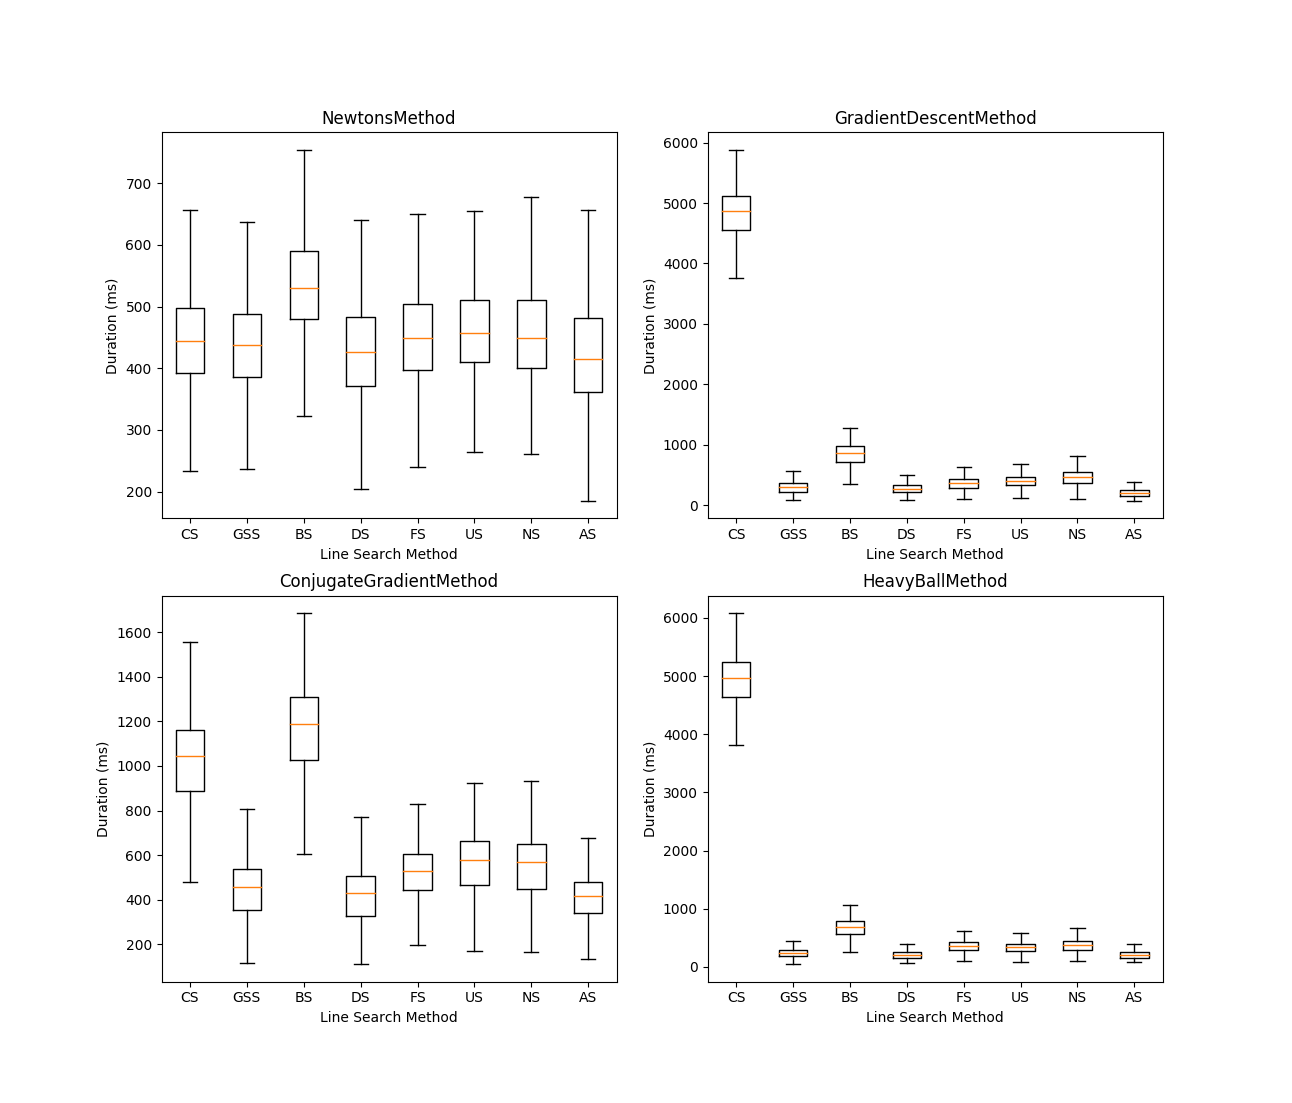
\includegraphics[width=1.0\textwidth]{images/boxplot_mss.png}
	\caption{Box plot of solution times per line search and main method for MatrixSquareSum target function.}
	\label{fig:boxplot_mss}
\end{figure}


\begin{figure}[H]
	\centering
	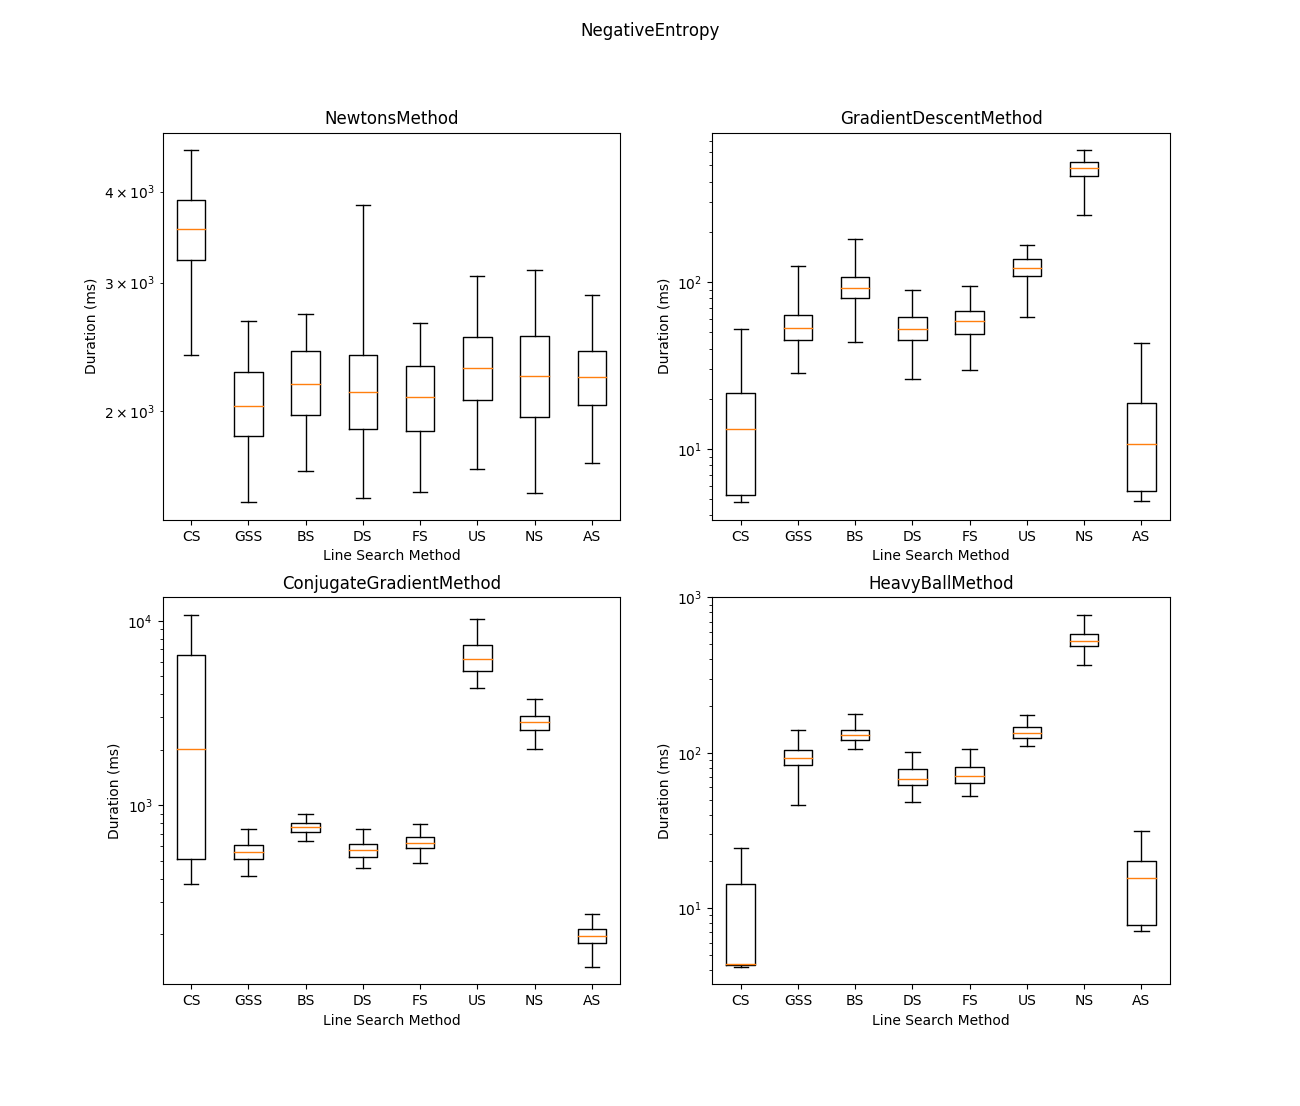
\includegraphics[width=1.0\textwidth]{images/boxplot_ne.png}
	\caption{Box plot of solution times per line search and main method for NegativeEntropy target function.}
	\label{fig:boxplot_ne}
\end{figure}

\todoinline{Explain the box plot method. Apparently the box contains 50\% of the dataset and the lines rest or smthing like that?}
\todoinline{Should I make separate boxplots with the best searches or something to improve the scale for their comparison?}
%https://matplotlib.org/3.1.1/gallery/statistics/boxplot_demo.html
%https://towardsdatascience.com/understanding-boxplots-5e2df7bcbd51


\subsubsection*{Constant Search}

Constant Search always gives a constant step size and therefore provides an excellent baseline to compare the other line search methods with. The execution of Constant Search costs zero time, so the burden of optimization remains on the main method.

Looking at the overall durations of Constant Search in table \ref{tab:colors_avg_overall} and the success rates in tables \ref{tab:colors_success_mss} and \ref{tab:colors_success_ne}, we can see that the Constant Search is generally the worst-performing method as expected. The only scenarios where constant step size proves to be rather effective are when optimizing the Negative Entropy function using Gradient Descent or Heavy Ball methods. In those two cases, the Constant Search was the best or second-best performer. With NE problem gradient descent based methods seem to perform well in general, and since the Constant Search does not require any time to execute, it gives high overall performances as well. We can confirm this conclusion by looking at the overall and line search duration columns in tables \ref{tab:performance_results_NE_GDM} and \ref{tab:performance_results_NE_HBM}, where most of the overall duration consists of the line search duration alone.

Looking at the box plots in figures \ref{fig:boxplot_mss} and \ref{fig:boxplot_ne} Constant Search is again the worst performer by not just absolute durations but also by the high variance of results. The only two exceptions to this are the previously mentioned cases of NE+GD and NE+HBM, where Constant Search scores one of the lowest variances.

\subsubsection*{Golden Section Search}

Comparing the overall results in tables \ref{tab:colors_avg_overall_mm} and \ref{tab:colors_avg_overall}, we immediately notice from the green-colored cells that Golden Section Search is one of the best performing line searches. The success rates of this method are great, and it does, like most methods tested, find the correct solution in almost all of the test cases. The variances of Golden Section Search's durations are approximately on the same level as the other line searches as can be seen from box plots.

\subsubsection*{Bisection Search}

Bisection Search does perform rather poorly in our test setup. It scores the second-lowest total success rate, though only losing by 0.4 percentile points to others in the single case of MSS+NM. The overall performance is especially weak with MSS problem and barely average with other setups, causing it to land around the middle of the scale of line search methods in the overall score table. The box plots also show that the Bisection Method does have higher variances in performance than other methods, especially with the MSS problem.

\subsubsection*{Dichotomous Search}

In our first tests, Dichotomous Search was one of the slower methods due to not reaching the correct solutions within the given max iteration limit. However, lowering the main method tolerance proved to be especially helpful for this method, which ultimately turned out as one of the stronger methods. It even outperforms Golden Section Search in MSS optimization and scores almost equally in overall scores. The success rates are also identical and reviewing variance from box plots shows no significant differences between the two methods sharing the second-best place in our comparison.

\subsubsection*{Fibonacci Search}

Fibonacci Search scores above-average in overall results and much higher with the NE problem when compared to other line searches. The success rates are in order and variances are at the same level as Dichotomous and Golden Section Searches'.

Our implementation of Fibonacci Search computes each Fibonacci number during runtime without memorizing them. The solution proved not to be an issue since the highest Fibonacci number reached was around $F_{50}$. A quick test with precomputed Fibonacci numbers showed at most 10\% improvement in performance when using memorization. For real-life applications, precomputation should probably be added if possible.

\subsubsection*{Uniform Search}

Uniform Search is expected to be slow since it is pretty straight forward and inefficient algorithm. The inefficiency can also be seen in the results as the algorithm scores averagely on MSS problem and below average in NE. Uniform Search also struggles to stay within the 10000 max iteration limit with NE problem when using Conjugate Gradient Method. This is possibly due to the way we implemented the positive domain using the Domain Limiter (algorithm \ref{alg:domain_limiter}). Uniform Search scores second-lowest in overall performance with average success rates and above-average variances.

\subsubsection*{Newton's Search}

Similarily to Uniform Search, Newton's Search has average performance when optimizing MSS problem but quickly falls behind in the case of NE. Newton's Search also seems to hit the max iterations limit with NE, but the method ends up still providing good enough step sizes so that success rates stay high. It seems that the method does not fully converge when combined with the domain limiter, which alters the step size given by the derivatives. Because of this, even though it does not make sense in real life implementation, a way smaller max iteration limit of just 100 or 1000 iterations proved to be much more effective for the NE problem. Because of this, the results of Newton's Search for NE are more unreliable than in the case of the MSS problem. The same effect is visible in the box plots as well: Newton's Search's durations have an extremely high variance when optimizing the Negative Entropy function.

\subsubsection*{Armijo's Search}

Armijo's Search proves to be the best overall performing method of the tested line searches. It has the best performance in five categories out of eight and is right on par with the top performers in the rest of the categories as well. It also has a slightly better success rate than any other method on MSS+GD and MSS+HBM test cases. Armijo's Search has a slightly higher variance in some scenarios than other line searches, but still easily outperforms other methods most of the time. Especially for NE problem, the Armijo's Search has lower variances than any other method.

\subsection{Assumptions and further performance improvements}

The assumptions and choices made during the research are discussed here briefly. One major factor affecting the results is that there are only two types of different optimization problems considered. Even though the randomization of parameters adds some variety in Matrix Square Sum problem, both of the target functions remain relatively simple. Both of the problems are also convex and have a single global maximum, making the solving easier than if there were multiple local maxima present. The way MSS's parameters are randomized is also a factor to consider. The methods for randomization of the parameters and building a positive-definite matrix $A$ described in section \ref{sect:matrix_square_sum} only yield a limited variety of functions. In the case of Negative Entropy, a domain limiter is used to ensure that values stay within the correct domain, which potentially causes issues with the line searches. Few line searches even struggled to converge at all in some scenarios.

Another factor to consider is the starting points used. While, in theory, we could raise the point count indefinitely, the solution for evenly distributing the points should provide decent results even with lower point counts. However, the range from which we generate the points could have been set higher than ten.

Choosing the optimal parameter values is also a significant factor in performance comparison. Since the problem of choosing the absolute best parameters is complex in itself, it is justified to pick a set of options and then compare the performance of each permutation. However, by implementing a better parameter selection, such as increasing the number of options, test cases, and iterations used, we can likely reach better results for each optimization method. The tradeoff would naturally be a higher computation time required to find the optimal parameters.

Some factors in performance are difficult to review accurately. These include the actual implementation of the methods which varies in different sources. One difference, in particular, seems to be the position of the stopping condition within the main methods. Some sources suggest that it is better to check the condition before updating the point. However, in our implementation, the check is done just after the update. \cite{book:convex_optimization} \cite{book:nonlinear_programming}

Another possible optimization is the pre-calculation of line search values. This means that we pre-evaluate and save the values for each different input for each line search so that instead of running the algorithm, we get the pre-evaluated value from our dictionary. \cite{book:convex_optimization}

Factors like the choice of programming language and CPU or GPU performance may affect the optimal results. We performed the tests in this thesis with Python 3.7.3 using a multiprocessing library and an Intel i5-8500K CPU. Different implementations and programming languages may, for example, optimize matrix calculations differently causing potentially unexpected differences within otherwise identical scenarios. For this reason, if the goal is to optimize the optimization process completely, it is suggested to run the performance testing separately for each test setup used.


\section{Conclusion and Future Research}


The choice of line search method seems to have a varying size of an impact on the performance of an optimization method. Comparing just the overall average duration caused by different line searches, it seems that the worst line search is several times slower than the best one. The difference in performance for the best and second-best method is around 11 \%, and the third one is around 16 \% slower than the fastest one.

For future research, we would suggest increasing the number of target functions and increasing the starting point value range. However, there is even more constraining issue we would need to tackle first: the optimal parameters are likely to change with the setups, forcing us to re-run the parameter comparisons and find new values for all the parameters. Since this requires high computation times, we should implement a better method for parameter selection before adding new target test scenarios. A simple solution could even be to decide a strict but well-reasoned set of few options for each parameter. We could base the value options, for example, on other previous research of the line search methods.

So, is it worth it to optimize the choice of line search method as an additional parameter of an unconstrained nonlinear optimization method? Judging by the results of this paper, we would say yes - sometimes. In particular, we believe the subject could use further research to make the results more comprehensive, but with the current results, we can show that there are indeed performance differences between the line searches. However, the results are not surprising, and the methods that we generally consider to be efficient are, in fact, the best choices in most use cases. There might exist problems for which some algorithms fit better than others, and therefore if the goal is to optimize a single problem as thoroughly as possible, the choice of line search method might be worth considering as an additional parameter. As long as a decent line search method is used in the first place, optimizing its parameters might be a better idea than looking for an alternative line search algorithm.

% %
% % LÄHDELUETTELO
% %  BibTeX-tiedoston kokoaminen onnistuu näppärästi esim. 
% %  Firefoxin Zotero-lisäosalla http://www.zotero.org/
% %  joka osaa poimia viitteet suoraan Google Scholarista.
% %
\newpage
% \bibliographystyle{plainnat}
\bibliographystyle{abbrvnat}
%\bibliographystyle{plain} % valitse tämä jos et käytä natbib-pakettia

% Ladataan library.bib
\bibliography{library}


% %
% % LIITTEET
% %

\newpage
\appendix
\section{Appendix}
\label{sect:appendix}
% TODO: enable

\subsection{Constant Search}
\begin{figure}[H]
\captionof{figure}{Best parameter permutations for different main methods using ConstantSearch for optimizing the MatrixSquareSum function with 10 sample points.}
\label{fig:param_comp_MatrixSquareSum_ConstantSearch}
\begin{subfigure}[ht]{.5\textwidth}
\rowcolors{2}{white}{gray!5}
\begin{tabular}{|c|c|c|}
\hline
\rowcolor{gray!25}
\multicolumn{3}{|c|}{NewtonsMethod} \\
\hline
\rowcolor{gray!25}
$(\lambda)$ & $s$ (\%) & $t$ (ms) \\
\hline
(1.0,) & 100.0 & 436.3 \\
(0.9,) & 100.0 & 4072.7 \\
(1.1,) & 100.0 & 4389.6 \\
(1.5,) & 100.0 & 11768.2 \\
(0.5,) & 100.0 & 13857.0 \\
\hline
\end{tabular}
\caption{Top 5 permutations with NewtonsMethod}
\label{subfig:param_comp_MatrixSquareSum_NewtonsMethod_ConstantSearch}
\end{subfigure}
\hfill
\begin{subfigure}[ht]{.5\textwidth}
\rowcolors{2}{white}{gray!5}
\begin{tabular}{|c|c|c|}
\hline
\rowcolor{gray!25}
\multicolumn{3}{|c|}{GradientDescentMethod} \\
\hline
\rowcolor{gray!25}
$(\lambda)$ & $s$ (\%) & $t$ (ms) \\
\hline
(0.0001,) & 100.0 & 8299.9 \\
(0.5,) & 0.0 & 162.8 \\
(0.9,) & 0.0 & 169.7 \\
(0.1,) & 0.0 & 187.9 \\
(0.25,) & 0.0 & 193.4 \\
\hline
\end{tabular}
\caption{Top 5 permutations with GradientDescentMethod}
\label{subfig:param_comp_MatrixSquareSum_GradientDescentMethod_ConstantSearch}
\end{subfigure}
\hfill
\begin{subfigure}[ht]{.5\textwidth}
\rowcolors{2}{white}{gray!5}
\begin{tabular}{|c|c|c|}
\hline
\rowcolor{gray!25}
\multicolumn{3}{|c|}{ConjugateGradientMethod} \\
\hline
\rowcolor{gray!25}
$(\lambda)$ & $s$ (\%) & $t$ (ms) \\
\hline
(0.0001,) & 100.0 & 1054.7 \\
(0.1,) & 0.0 & 192.4 \\
(0.5,) & 0.0 & 270.2 \\
(0.25,) & 0.0 & 280.1 \\
(0.9,) & 0.0 & 298.0 \\
\hline
\end{tabular}
\caption{Top 5 permutations with ConjugateGradientMethod}
\label{subfig:param_comp_MatrixSquareSum_ConjugateGradientMethod_ConstantSearch}
\end{subfigure}
\hfill
\begin{subfigure}[ht]{.5\textwidth}
\rowcolors{2}{white}{gray!5}
\begin{tabular}{|c|c|c|}
\hline
\rowcolor{gray!25}
\multicolumn{3}{|c|}{HeavyBallMethod} \\
\hline
\rowcolor{gray!25}
$(\lambda,\beta_{HBM})$ & $s$ (\%) & $t$ (ms) \\
\hline
(0.0001, 0.1) & 100.0 & 6437.8 \\
(0.0001, 0.5) & 100.0 & 6580.6 \\
(0.0001, 10.0) & 100.0 & 6714.6 \\
(0.0001, 5.0) & 100.0 & 6784.6 \\
(0.0001, 1.0) & 100.0 & 6838.7 \\
\hline
\end{tabular}
\caption{Top 5 permutations with HeavyBallMethod}
\label{subfig:param_comp_MatrixSquareSum_HeavyBallMethod_ConstantSearch}
\end{subfigure}
\end{figure}

\begin{figure}[H]
\captionof{figure}{Best parameter permutations for different main methods using ConstantSearch for optimizing the NegativeEntropy function with 10 sample points.}
\label{fig:param_comp_NegativeEntropy_ConstantSearch}
\begin{subfigure}[ht]{.5\textwidth}
\rowcolors{2}{white}{gray!5}
\begin{tabular}{|c|c|c|}
\hline
\rowcolor{gray!25}
\multicolumn{3}{|c|}{NewtonsMethod} \\
\hline
\rowcolor{gray!25}
$(\lambda)$ & $s$ (\%) & $t$ (ms) \\
\hline
(0.9,) & 100.0 & 3379.7 \\
(0.5,) & 100.0 & 7239.4 \\
(0.25,) & 100.0 & 17055.7 \\
(0.1,) & 100.0 & 46295.4 \\
\hline
\end{tabular}
\caption{Top 5 permutations with NewtonsMethod}
\label{subfig:param_comp_NegativeEntropy_NewtonsMethod_ConstantSearch}
\end{subfigure}
\hfill
\begin{subfigure}[ht]{.5\textwidth}
\rowcolors{2}{white}{gray!5}
\begin{tabular}{|c|c|c|}
\hline
\rowcolor{gray!25}
\multicolumn{3}{|c|}{GradientDescentMethod} \\
\hline
\rowcolor{gray!25}
$(\lambda)$ & $s$ (\%) & $t$ (ms) \\
\hline
(0.5,) & 100.0 & 17.8 \\
(0.25,) & 100.0 & 57.5 \\
(0.1,) & 100.0 & 226.9 \\
\hline
\end{tabular}
\caption{Top 5 permutations with GradientDescentMethod}
\label{subfig:param_comp_NegativeEntropy_GradientDescentMethod_ConstantSearch}
\end{subfigure}
\hfill
\begin{subfigure}[ht]{.5\textwidth}
\rowcolors{2}{white}{gray!5}
\begin{tabular}{|c|c|c|}
\hline
\rowcolor{gray!25}
\multicolumn{3}{|c|}{ConjugateGradientMethod} \\
\hline
\rowcolor{gray!25}
$(\lambda)$ & $s$ (\%) & $t$ (ms) \\
\hline
(0.1,) & 100.0 & 2361.4 \\
(0.0001,) & 100.0 & 4281.1 \\
(0.15,) & 100.0 & 4969.4 \\
(0.2,) & 100.0 & 6062.7 \\
\hline
\end{tabular}
\caption{Top 5 permutations with ConjugateGradientMethod}
\label{subfig:param_comp_NegativeEntropy_ConjugateGradientMethod_ConstantSearch}
\end{subfigure}
\hfill
\begin{subfigure}[ht]{.5\textwidth}
\rowcolors{2}{white}{gray!5}
\begin{tabular}{|c|c|c|}
\hline
\rowcolor{gray!25}
\multicolumn{3}{|c|}{HeavyBallMethod} \\
\hline
\rowcolor{gray!25}
$(\lambda,\beta_{HBM})$ & $s$ (\%) & $t$ (ms) \\
\hline
(0.5, 0.1) & 100.0 & 9.1 \\
(0.5, 0.5) & 100.0 & 14.7 \\
(0.25, 0.1) & 100.0 & 15.3 \\
(0.25, 0.5) & 100.0 & 15.8 \\
(0.25, 1.0) & 100.0 & 18.2 \\
\hline
\end{tabular}
\caption{Top 5 permutations with HeavyBallMethod}
\label{subfig:param_comp_NegativeEntropy_HeavyBallMethod_ConstantSearch}
\end{subfigure}
\end{figure}

\subsection{Golden Section Search}
\begin{center}
\rowcolors{2}{white}{gray!5}
\captionof{table}{Parameters tested for GoldenSectionSearch}
\label{tab:params_GoldenSectionSearch}
\begin{tabular}{|c|c|c|}
\hline
\rowcolor{gray!25}
Parameter & MatrixSquareSum & NegativeEntropy \\
\hline
$a$ & -10, -5 & -10, -5 \\
$b$ & 10, 5 & 10, 5 \\
$l$ & 0.0001, 1e-07 & 0.0001, 1e-07 \\
\hline
\end{tabular}
\end{center}

\begin{figure}[H]
\captionof{figure}{Best parameter permutations for different main methods using GoldenSectionSearch for optimizing the MatrixSquareSum function with 10 sample points.}
\label{fig:param_comp_MatrixSquareSum_GoldenSectionSearch}
\begin{subfigure}[ht]{.5\textwidth}
\rowcolors{2}{white}{gray!5}
\begin{tabular}{|c|c|c|}
\hline
\rowcolor{gray!25}
\multicolumn{3}{|c|}{NewtonsMethod} \\
\hline
\rowcolor{gray!25}
$(a,b,l)$ & $s$ (\%) & $t$ (ms) \\
\hline
(-10, 5, 1e-07) & 100.0 & 515.6 \\
(-10, 10, 1e-07) & 100.0 & 868.6 \\
(-10, 10, 0.0001) & 100.0 & 887.5 \\
(-5, 5, 1e-07) & 100.0 & 891.0 \\
(-5, 10, 0.0001) & 100.0 & 914.0 \\
\hline
\end{tabular}
\caption{Top 5 permutations with NewtonsMethod}
\label{subfig:param_comp_MatrixSquareSum_NewtonsMethod_GoldenSectionSearch}
\end{subfigure}
\hfill
\begin{subfigure}[ht]{.5\textwidth}
\rowcolors{2}{white}{gray!5}
\begin{tabular}{|c|c|c|}
\hline
\rowcolor{gray!25}
\multicolumn{3}{|c|}{GradientDescentMethod} \\
\hline
\rowcolor{gray!25}
$(a,b,l)$ & $s$ (\%) & $t$ (ms) \\
\hline
(-10, 5, 0.0001) & 100.0 & 279.4 \\
(-5, 10, 0.0001) & 100.0 & 318.0 \\
(-5, 5, 0.0001) & 100.0 & 344.3 \\
(-10, 5, 1e-07) & 100.0 & 371.1 \\
(-10, 10, 0.0001) & 100.0 & 379.6 \\
\hline
\end{tabular}
\caption{Top 5 permutations with GradientDescentMethod}
\label{subfig:param_comp_MatrixSquareSum_GradientDescentMethod_GoldenSectionSearch}
\end{subfigure}
\hfill
\begin{subfigure}[ht]{.5\textwidth}
\rowcolors{2}{white}{gray!5}
\begin{tabular}{|c|c|c|}
\hline
\rowcolor{gray!25}
\multicolumn{3}{|c|}{ConjugateGradientMethod} \\
\hline
\rowcolor{gray!25}
$(a,b,l)$ & $s$ (\%) & $t$ (ms) \\
\hline
(-5, 10, 0.0001) & 100.0 & 436.7 \\
(-10, 10, 0.0001) & 100.0 & 467.8 \\
(-5, 5, 0.0001) & 100.0 & 489.2 \\
(-10, 5, 0.0001) & 100.0 & 529.8 \\
(-10, 10, 1e-07) & 100.0 & 533.9 \\
\hline
\end{tabular}
\caption{Top 5 permutations with ConjugateGradientMethod}
\label{subfig:param_comp_MatrixSquareSum_ConjugateGradientMethod_GoldenSectionSearch}
\end{subfigure}
\hfill
\begin{subfigure}[ht]{.5\textwidth}
\rowcolors{2}{white}{gray!5}
\begin{tabular}{|c|c|c|}
\hline
\rowcolor{gray!25}
\multicolumn{3}{|c|}{HeavyBallMethod} \\
\hline
\rowcolor{gray!25}
$(a,b,l,\beta_{HBM})$ & $s$ (\%) & $t$ (ms) \\
\hline
(-5, 10, 0.0001, 10.0) & 100.0 & 230.6 \\
(-10, 5, 0.0001, 10.0) & 100.0 & 236.7 \\
(-10, 10, 0.0001, 10.0) & 100.0 & 243.6 \\
(-5, 10, 0.0001, 5.0) & 100.0 & 244.8 \\
(-5, 5, 0.0001, 10.0) & 100.0 & 252.1 \\
\hline
\end{tabular}
\caption{Top 5 permutations with HeavyBallMethod}
\label{subfig:param_comp_MatrixSquareSum_HeavyBallMethod_GoldenSectionSearch}
\end{subfigure}
\end{figure}

\begin{figure}[H]
\captionof{figure}{Best parameter permutations for different main methods using GoldenSectionSearch for optimizing the NegativeEntropy function with 10 sample points.}
\label{fig:param_comp_NegativeEntropy_GoldenSectionSearch}
\begin{subfigure}[ht]{.5\textwidth}
\rowcolors{2}{white}{gray!5}
\begin{tabular}{|c|c|c|}
\hline
\rowcolor{gray!25}
\multicolumn{3}{|c|}{NewtonsMethod} \\
\hline
\rowcolor{gray!25}
$(a,b,l)$ & $s$ (\%) & $t$ (ms) \\
\hline
(-5, 5, 1e-07) & 100.0 & 1758.0 \\
(-10, 5, 0.0001) & 100.0 & 1905.6 \\
(-10, 10, 0.0001) & 100.0 & 1946.7 \\
(-10, 10, 1e-07) & 100.0 & 1947.3 \\
(-5, 5, 0.0001) & 100.0 & 1968.5 \\
\hline
\end{tabular}
\caption{Top 5 permutations with NewtonsMethod}
\label{subfig:param_comp_NegativeEntropy_NewtonsMethod_GoldenSectionSearch}
\end{subfigure}
\hfill
\begin{subfigure}[ht]{.5\textwidth}
\rowcolors{2}{white}{gray!5}
\begin{tabular}{|c|c|c|}
\hline
\rowcolor{gray!25}
\multicolumn{3}{|c|}{GradientDescentMethod} \\
\hline
\rowcolor{gray!25}
$(a,b,l)$ & $s$ (\%) & $t$ (ms) \\
\hline
(-5, 5, 0.0001) & 100.0 & 57.1 \\
(-5, 5, 1e-07) & 100.0 & 68.4 \\
(-5, 10, 0.0001) & 100.0 & 85.4 \\
(-5, 10, 1e-07) & 100.0 & 85.8 \\
(-10, 5, 1e-07) & 100.0 & 109.9 \\
\hline
\end{tabular}
\caption{Top 5 permutations with GradientDescentMethod}
\label{subfig:param_comp_NegativeEntropy_GradientDescentMethod_GoldenSectionSearch}
\end{subfigure}
\hfill
\begin{subfigure}[ht]{.5\textwidth}
\rowcolors{2}{white}{gray!5}
\begin{tabular}{|c|c|c|}
\hline
\rowcolor{gray!25}
\multicolumn{3}{|c|}{ConjugateGradientMethod} \\
\hline
\rowcolor{gray!25}
$(a,b,l)$ & $s$ (\%) & $t$ (ms) \\
\hline
(-5, 5, 0.0001) & 100.0 & 591.3 \\
(-10, 5, 0.0001) & 100.0 & 644.1 \\
(-5, 5, 1e-07) & 100.0 & 644.4 \\
(-5, 10, 0.0001) & 100.0 & 648.5 \\
(-10, 5, 1e-07) & 100.0 & 672.1 \\
\hline
\end{tabular}
\caption{Top 5 permutations with ConjugateGradientMethod}
\label{subfig:param_comp_NegativeEntropy_ConjugateGradientMethod_GoldenSectionSearch}
\end{subfigure}
\hfill
\begin{subfigure}[ht]{.5\textwidth}
\rowcolors{2}{white}{gray!5}
\begin{tabular}{|c|c|c|}
\hline
\rowcolor{gray!25}
\multicolumn{3}{|c|}{HeavyBallMethod} \\
\hline
\rowcolor{gray!25}
$(a,b,l,\beta_{HBM})$ & $s$ (\%) & $t$ (ms) \\
\hline
(-5, 5, 0.0001, 0.1) & 100.0 & 72.3 \\
(-10, 5, 0.0001, 0.1) & 100.0 & 75.0 \\
(-5, 10, 0.0001, 0.1) & 100.0 & 75.2 \\
(-5, 5, 1e-07, 0.1) & 100.0 & 79.7 \\
(-5, 10, 1e-07, 0.1) & 100.0 & 80.4 \\
\hline
\end{tabular}
\caption{Top 5 permutations with HeavyBallMethod}
\label{subfig:param_comp_NegativeEntropy_HeavyBallMethod_GoldenSectionSearch}
\end{subfigure}
\end{figure}

\subsection{Bisection Search}
\begin{figure}[H]
\captionof{figure}{Best parameter permutations for different main methods using BisectionSearch for optimizing the MatrixSquareSum function with 10 sample points.}
\label{fig:param_comp_MatrixSquareSum_BisectionSearch}
\begin{subfigure}[ht]{.5\textwidth}
\rowcolors{2}{white}{gray!5}
\begin{tabular}{|c|c|c|}
\hline
\rowcolor{gray!25}
\multicolumn{3}{|c|}{NewtonsMethod} \\
\hline
\rowcolor{gray!25}
$(a,b,l)$ & $s$ (\%) & $t$ (ms) \\
\hline
(-10, 5, 1e-07) & 100.0 & 555.4 \\
(-5, 10, 1e-07) & 100.0 & 597.9 \\
(-5, 5, 1e-07) & 100.0 & 962.4 \\
(-10, 5, 0.0001) & 100.0 & 1025.9 \\
(-10, 10, 0.0001) & 100.0 & 1049.4 \\
\hline
\end{tabular}
\caption{Top 5 permutations with NewtonsMethod}
\label{subfig:param_comp_MatrixSquareSum_NewtonsMethod_BisectionSearch}
\end{subfigure}
\hfill
\begin{subfigure}[ht]{.5\textwidth}
\rowcolors{2}{white}{gray!5}
\begin{tabular}{|c|c|c|}
\hline
\rowcolor{gray!25}
\multicolumn{3}{|c|}{GradientDescentMethod} \\
\hline
\rowcolor{gray!25}
$(a,b,l)$ & $s$ (\%) & $t$ (ms) \\
\hline
(-10, 5, 0.0001) & 100.0 & 836.1 \\
(-5, 5, 0.0001) & 100.0 & 911.2 \\
(-10, 10, 0.0001) & 100.0 & 921.0 \\
(-5, 10, 0.0001) & 100.0 & 956.1 \\
(-5, 5, 1e-07) & 100.0 & 1094.3 \\
\hline
\end{tabular}
\caption{Top 5 permutations with GradientDescentMethod}
\label{subfig:param_comp_MatrixSquareSum_GradientDescentMethod_BisectionSearch}
\end{subfigure}
\hfill
\begin{subfigure}[ht]{.5\textwidth}
\rowcolors{2}{white}{gray!5}
\begin{tabular}{|c|c|c|}
\hline
\rowcolor{gray!25}
\multicolumn{3}{|c|}{ConjugateGradientMethod} \\
\hline
\rowcolor{gray!25}
$(a,b,l)$ & $s$ (\%) & $t$ (ms) \\
\hline
(-10, 10, 0.0001) & 100.0 & 1152.1 \\
(-5, 5, 0.0001) & 100.0 & 1153.7 \\
(-10, 5, 0.0001) & 100.0 & 1157.4 \\
(-5, 10, 0.0001) & 100.0 & 1175.7 \\
(-5, 10, 1e-07) & 100.0 & 1575.7 \\
\hline
\end{tabular}
\caption{Top 5 permutations with ConjugateGradientMethod}
\label{subfig:param_comp_MatrixSquareSum_ConjugateGradientMethod_BisectionSearch}
\end{subfigure}
\hfill
\begin{subfigure}[ht]{.5\textwidth}
\rowcolors{2}{white}{gray!5}
\begin{tabular}{|c|c|c|}
\hline
\rowcolor{gray!25}
\multicolumn{3}{|c|}{HeavyBallMethod} \\
\hline
\rowcolor{gray!25}
$(a,b,l,\beta_{HBM})$ & $s$ (\%) & $t$ (ms) \\
\hline
(-10, 10, 0.0001, 10.0) & 100.0 & 581.2 \\
(-5, 10, 0.0001, 5.0) & 100.0 & 627.6 \\
(-5, 10, 0.0001, 10.0) & 100.0 & 676.6 \\
(-5, 5, 0.0001, 10.0) & 100.0 & 706.7 \\
(-5, 5, 0.0001, 5.0) & 100.0 & 714.3 \\
\hline
\end{tabular}
\caption{Top 5 permutations with HeavyBallMethod}
\label{subfig:param_comp_MatrixSquareSum_HeavyBallMethod_BisectionSearch}
\end{subfigure}
\end{figure}

\begin{figure}[H]
\captionof{figure}{Best parameter permutations for different main methods using BisectionSearch for optimizing the NegativeEntropy function with 10 sample points.}
\label{fig:param_comp_NegativeEntropy_BisectionSearch}
\begin{subfigure}[ht]{.5\textwidth}
\rowcolors{2}{white}{gray!5}
\begin{tabular}{|c|c|c|}
\hline
\rowcolor{gray!25}
\multicolumn{3}{|c|}{NewtonsMethod} \\
\hline
\rowcolor{gray!25}
$(a,b,l)$ & $s$ (\%) & $t$ (ms) \\
\hline
(-10, 10, 0.0001) & 100.0 & 1753.5 \\
(-10, 5, 0.0001) & 100.0 & 2006.3 \\
(-5, 5, 1e-07) & 100.0 & 2044.7 \\
(-5, 10, 0.0001) & 100.0 & 2075.4 \\
(-5, 5, 0.0001) & 100.0 & 2162.0 \\
\hline
\end{tabular}
\caption{Top 5 permutations with NewtonsMethod}
\label{subfig:param_comp_NegativeEntropy_NewtonsMethod_BisectionSearch}
\end{subfigure}
\hfill
\begin{subfigure}[ht]{.5\textwidth}
\rowcolors{2}{white}{gray!5}
\begin{tabular}{|c|c|c|}
\hline
\rowcolor{gray!25}
\multicolumn{3}{|c|}{GradientDescentMethod} \\
\hline
\rowcolor{gray!25}
$(a,b,l)$ & $s$ (\%) & $t$ (ms) \\
\hline
(-5, 5, 0.0001) & 100.0 & 105.5 \\
(-10, 5, 0.0001) & 100.0 & 114.6 \\
(-5, 10, 0.0001) & 100.0 & 115.6 \\
(-10, 5, 1e-07) & 100.0 & 128.9 \\
(-5, 5, 1e-07) & 100.0 & 136.3 \\
\hline
\end{tabular}
\caption{Top 5 permutations with GradientDescentMethod}
\label{subfig:param_comp_NegativeEntropy_GradientDescentMethod_BisectionSearch}
\end{subfigure}
\hfill
\begin{subfigure}[ht]{.5\textwidth}
\rowcolors{2}{white}{gray!5}
\begin{tabular}{|c|c|c|}
\hline
\rowcolor{gray!25}
\multicolumn{3}{|c|}{ConjugateGradientMethod} \\
\hline
\rowcolor{gray!25}
$(a,b,l)$ & $s$ (\%) & $t$ (ms) \\
\hline
(-5, 5, 0.0001) & 100.0 & 883.4 \\
(-10, 10, 0.0001) & 100.0 & 891.5 \\
(-10, 5, 0.0001) & 100.0 & 893.8 \\
(-5, 10, 0.0001) & 100.0 & 916.2 \\
(-10, 5, 1e-07) & 100.0 & 1092.6 \\
\hline
\end{tabular}
\caption{Top 5 permutations with ConjugateGradientMethod}
\label{subfig:param_comp_NegativeEntropy_ConjugateGradientMethod_BisectionSearch}
\end{subfigure}
\hfill
\begin{subfigure}[ht]{.5\textwidth}
\rowcolors{2}{white}{gray!5}
\begin{tabular}{|c|c|c|}
\hline
\rowcolor{gray!25}
\multicolumn{3}{|c|}{HeavyBallMethod} \\
\hline
\rowcolor{gray!25}
$(a,b,l,\beta_{HBM})$ & $s$ (\%) & $t$ (ms) \\
\hline
(-10, 10, 0.0001, 0.1) & 100.0 & 138.9 \\
(-5, 5, 0.0001, 0.1) & 100.0 & 142.4 \\
(-10, 5, 0.0001, 0.1) & 100.0 & 153.4 \\
(-5, 10, 0.0001, 0.1) & 100.0 & 154.3 \\
(-5, 5, 0.0001, 0.5) & 100.0 & 182.9 \\
\hline
\end{tabular}
\caption{Top 5 permutations with HeavyBallMethod}
\label{subfig:param_comp_NegativeEntropy_HeavyBallMethod_BisectionSearch}
\end{subfigure}
\end{figure}

\subsection{Dichotomous Search}
\begin{figure}[H]
\captionof{figure}{Best parameter permutations for different main methods using DichotomousSearch for optimizing the MatrixSquareSum function with 10 sample points.}
\label{fig:param_comp_MatrixSquareSum_DichotomousSearch}
\makebox[\linewidth][c]{
\begin{subfigure}[ht]{.6\textwidth}
\centering
\rowcolors{2}{white}{gray!5}
\begin{tabular}{|c|c|c|}
\hline
\rowcolor{gray!25}
\multicolumn{3}{|c|}{NewtonsMethod} \\
\hline
\rowcolor{gray!25}
$(a,b,\epsilon,l)$ & $s$ (\%) & $t$ (ms) \\
\hline
(-5, 10, 1e-10, 1e-09) & 100.0 & 388.3 \\
(-10, 10, 1e-10, 1e-09) & 100.0 & 436.4 \\
(-5, 5, 1e-10, 1e-09) & 100.0 & 439.6 \\
(-10, 5, 1e-10, 1e-09) & 100.0 & 455.0 \\
(-5, 10, 1e-07, 1e-05) & 100.0 & 840.8 \\
\hline
\end{tabular}
\caption{Top 5 permutations with NewtonsMethod}
\label{subfig:param_comp_MatrixSquareSum_NewtonsMethod_DichotomousSearch}
\end{subfigure}
\hfill
\begin{subfigure}[ht]{.6\textwidth}
\centering
\rowcolors{2}{white}{gray!5}
\begin{tabular}{|c|c|c|}
\hline
\rowcolor{gray!25}
\multicolumn{3}{|c|}{GradientDescentMethod} \\
\hline
\rowcolor{gray!25}
$(a,b,\epsilon,l)$ & $s$ (\%) & $t$ (ms) \\
\hline
(-10, 5, 1e-07, 1e-05) & 100.0 & 234.8 \\
(-10, 5, 1e-08, 0.0001) & 100.0 & 241.2 \\
(-5, 5, 1e-07, 0.0001) & 100.0 & 252.5 \\
(-5, 10, 1e-08, 0.0001) & 100.0 & 252.9 \\
(-10, 5, 1e-08, 1e-05) & 100.0 & 260.4 \\
\hline
\end{tabular}
\caption{Top 5 permutations with GradientDescentMethod}
\label{subfig:param_comp_MatrixSquareSum_GradientDescentMethod_DichotomousSearch}
\end{subfigure}
}
\makebox[\linewidth][c]{
\begin{subfigure}[ht]{.6\textwidth}
\centering
\rowcolors{2}{white}{gray!5}
\begin{tabular}{|c|c|c|}
\hline
\rowcolor{gray!25}
\multicolumn{3}{|c|}{ConjugateGradientMethod} \\
\hline
\rowcolor{gray!25}
$(a,b,\epsilon,l)$ & $s$ (\%) & $t$ (ms) \\
\hline
(-5, 10, 1e-07, 1e-05) & 100.0 & 354.2 \\
(-5, 10, 1e-07, 0.0001) & 100.0 & 382.0 \\
(-5, 5, 1e-07, 0.0001) & 100.0 & 397.3 \\
(-10, 10, 1e-08, 1e-05) & 100.0 & 406.2 \\
(-10, 5, 1e-08, 0.0001) & 100.0 & 406.7 \\
\hline
\end{tabular}
\caption{Top 5 permutations with ConjugateGradientMethod}
\label{subfig:param_comp_MatrixSquareSum_ConjugateGradientMethod_DichotomousSearch}
\end{subfigure}
\hfill
\begin{subfigure}[ht]{.6\textwidth}
\centering
\rowcolors{2}{white}{gray!5}
\begin{tabular}{|c|c|c|}
\hline
\rowcolor{gray!25}
\multicolumn{3}{|c|}{HeavyBallMethod} \\
\hline
\rowcolor{gray!25}
$(a,b,\epsilon,l,\beta_{HBM})$ & $s$ (\%) & $t$ (ms) \\
\hline
(-5, 5, 1e-07, 0.0001, 10.0) & 100.0 & 173.6 \\
(-10, 10, 1e-07, 0.0001, 10.0) & 100.0 & 185.4 \\
(-5, 10, 1e-08, 0.0001, 10.0) & 100.0 & 193.9 \\
(-10, 5, 1e-08, 1e-05, 5.0) & 100.0 & 202.6 \\
(-5, 5, 1e-07, 1e-05, 10.0) & 100.0 & 205.2 \\
\hline
\end{tabular}
\caption{Top 5 permutations with HeavyBallMethod}
\label{subfig:param_comp_MatrixSquareSum_HeavyBallMethod_DichotomousSearch}
\end{subfigure}
}
\end{figure}

\begin{figure}[H]
\captionof{figure}{Best parameter permutations for different main methods using DichotomousSearch for optimizing the NegativeEntropy function with 10 sample points.}
\label{fig:param_comp_NegativeEntropy_DichotomousSearch}
\makebox[\linewidth][c]{
\begin{subfigure}[ht]{.6\textwidth}
\centering
\rowcolors{2}{white}{gray!5}
\begin{tabular}{|c|c|c|}
\hline
\rowcolor{gray!25}
\multicolumn{3}{|c|}{NewtonsMethod} \\
\hline
\rowcolor{gray!25}
$(a,b,\epsilon,l)$ & $s$ (\%) & $t$ (ms) \\
\hline
(-10, 10, 1e-07, 1e-05) & 100.0 & 1756.0 \\
(-10, 5, 1e-06, 1e-05) & 100.0 & 1846.8 \\
(-10, 10, 1e-06, 0.0001) & 100.0 & 1882.9 \\
(-10, 5, 1e-06, 0.0001) & 100.0 & 1893.5 \\
(-10, 10, 1e-06, 1e-05) & 100.0 & 1923.0 \\
\hline
\end{tabular}
\caption{Top 5 permutations with NewtonsMethod}
\label{subfig:param_comp_NegativeEntropy_NewtonsMethod_DichotomousSearch}
\end{subfigure}
\hfill
\begin{subfigure}[ht]{.6\textwidth}
\centering
\rowcolors{2}{white}{gray!5}
\begin{tabular}{|c|c|c|}
\hline
\rowcolor{gray!25}
\multicolumn{3}{|c|}{GradientDescentMethod} \\
\hline
\rowcolor{gray!25}
$(a,b,\epsilon,l)$ & $s$ (\%) & $t$ (ms) \\
\hline
(-5, 5, 1e-07, 0.0001) & 100.0 & 54.3 \\
(-5, 10, 1e-06, 0.0001) & 100.0 & 61.7 \\
(-5, 10, 1e-06, 1e-05) & 100.0 & 63.8 \\
(-5, 5, 1e-07, 1e-05) & 100.0 & 64.6 \\
(-5, 10, 1e-07, 0.0001) & 100.0 & 65.4 \\
\hline
\end{tabular}
\caption{Top 5 permutations with GradientDescentMethod}
\label{subfig:param_comp_NegativeEntropy_GradientDescentMethod_DichotomousSearch}
\end{subfigure}
}
\makebox[\linewidth][c]{
\begin{subfigure}[ht]{.6\textwidth}
\centering
\rowcolors{2}{white}{gray!5}
\begin{tabular}{|c|c|c|}
\hline
\rowcolor{gray!25}
\multicolumn{3}{|c|}{ConjugateGradientMethod} \\
\hline
\rowcolor{gray!25}
$(a,b,\epsilon,l)$ & $s$ (\%) & $t$ (ms) \\
\hline
(-5, 5, 1e-06, 0.0001) & 100.0 & 640.6 \\
(-10, 5, 1e-06, 0.0001) & 100.0 & 642.7 \\
(-5, 5, 1e-07, 0.0001) & 100.0 & 645.3 \\
(-5, 10, 1e-07, 0.0001) & 100.0 & 657.0 \\
(-5, 5, 1e-06, 1e-05) & 100.0 & 680.9 \\
\hline
\end{tabular}
\caption{Top 5 permutations with ConjugateGradientMethod}
\label{subfig:param_comp_NegativeEntropy_ConjugateGradientMethod_DichotomousSearch}
\end{subfigure}
\hfill
\begin{subfigure}[ht]{.6\textwidth}
\centering
\rowcolors{2}{white}{gray!5}
\begin{tabular}{|c|c|c|}
\hline
\rowcolor{gray!25}
\multicolumn{3}{|c|}{HeavyBallMethod} \\
\hline
\rowcolor{gray!25}
$(a,b,\epsilon,l,\beta_{HBM})$ & $s$ (\%) & $t$ (ms) \\
\hline
(-5, 5, 1e-06, 1e-05, 0.1) & 100.0 & 70.4 \\
(-5, 5, 1e-06, 0.0001, 0.1) & 100.0 & 70.8 \\
(-10, 5, 1e-07, 0.0001, 0.1) & 100.0 & 73.3 \\
(-5, 10, 1e-06, 0.0001, 0.1) & 100.0 & 74.0 \\
(-5, 5, 1e-07, 0.0001, 0.1) & 100.0 & 74.0 \\
\hline
\end{tabular}
\caption{Top 5 permutations with HeavyBallMethod}
\label{subfig:param_comp_NegativeEntropy_HeavyBallMethod_DichotomousSearch}
\end{subfigure}
}
\end{figure}

\subsection{Fibonacci Search}
\begin{figure}[H]
\captionof{figure}{Best parameter permutations for different main methods using FibonacciSearch for optimizing the MatrixSquareSum function with 10 sample points.}
\label{fig:param_comp_MatrixSquareSum_FibonacciSearch}
\makebox[\linewidth][c]{
\begin{subfigure}[ht]{.6\textwidth}
\centering
\rowcolors{2}{white}{gray!5}
\begin{tabular}{|c|c|c|}
\hline
\rowcolor{gray!25}
\multicolumn{3}{|c|}{NewtonsMethod} \\
\hline
\rowcolor{gray!25}
$(a,b,\epsilon,l)$ & $s$ (\%) & $t$ (ms) \\
\hline
(-5, 5, 1e-10, 1e-10) & 100.0 & 443.2 \\
(-5, 5, 1e-12, 1e-10) & 100.0 & 452.3 \\
(-5, 5, 1e-08, 1e-10) & 100.0 & 459.6 \\
(-10, 5, 1e-10, 1e-10) & 100.0 & 460.9 \\
(-10, 5, 1e-12, 1e-10) & 100.0 & 469.7 \\
\hline
\end{tabular}
\caption{Top 5 permutations with NewtonsMethod}
\label{subfig:param_comp_MatrixSquareSum_NewtonsMethod_FibonacciSearch}
\end{subfigure}
\hfill
\begin{subfigure}[ht]{.6\textwidth}
\centering
\rowcolors{2}{white}{gray!5}
\begin{tabular}{|c|c|c|}
\hline
\rowcolor{gray!25}
\multicolumn{3}{|c|}{GradientDescentMethod} \\
\hline
\rowcolor{gray!25}
$(a,b,\epsilon,l)$ & $s$ (\%) & $t$ (ms) \\
\hline
(-5, 10, 1e-12, 1e-06) & 100.0 & 355.6 \\
(-5, 10, 1e-10, 1e-06) & 100.0 & 356.0 \\
(-5, 5, 1e-12, 1e-06) & 100.0 & 366.8 \\
(-10, 10, 1e-12, 1e-06) & 100.0 & 369.2 \\
(-10, 5, 1e-12, 1e-06) & 100.0 & 369.4 \\
\hline
\end{tabular}
\caption{Top 5 permutations with GradientDescentMethod}
\label{subfig:param_comp_MatrixSquareSum_GradientDescentMethod_FibonacciSearch}
\end{subfigure}
}
\makebox[\linewidth][c]{
\begin{subfigure}[ht]{.6\textwidth}
\centering
\rowcolors{2}{white}{gray!5}
\begin{tabular}{|c|c|c|}
\hline
\rowcolor{gray!25}
\multicolumn{3}{|c|}{ConjugateGradientMethod} \\
\hline
\rowcolor{gray!25}
$(a,b,\epsilon,l)$ & $s$ (\%) & $t$ (ms) \\
\hline
(-5, 10, 1e-10, 1e-06) & 100.0 & 473.8 \\
(-10, 10, 1e-10, 1e-06) & 100.0 & 485.0 \\
(-5, 10, 1e-12, 1e-06) & 100.0 & 490.3 \\
(-10, 5, 1e-08, 1e-06) & 100.0 & 508.6 \\
(-10, 10, 1e-12, 1e-06) & 100.0 & 516.0 \\
\hline
\end{tabular}
\caption{Top 5 permutations with ConjugateGradientMethod}
\label{subfig:param_comp_MatrixSquareSum_ConjugateGradientMethod_FibonacciSearch}
\end{subfigure}
\hfill
\begin{subfigure}[ht]{.6\textwidth}
\centering
\rowcolors{2}{white}{gray!5}
\begin{tabular}{|c|c|c|}
\hline
\rowcolor{gray!25}
\multicolumn{3}{|c|}{HeavyBallMethod} \\
\hline
\rowcolor{gray!25}
$(a,b,\epsilon,l,\beta_{HBM})$ & $s$ (\%) & $t$ (ms) \\
\hline
(-10, 5, 1e-12, 1e-06, 10.0) & 100.0 & 251.4 \\
(-5, 5, 1e-12, 1e-06, 10.0) & 100.0 & 268.5 \\
(-5, 5, 1e-08, 1e-06, 10.0) & 100.0 & 273.0 \\
(-10, 10, 1e-12, 1e-06, 10.0) & 100.0 & 273.5 \\
(-5, 5, 1e-10, 1e-06, 10.0) & 100.0 & 273.5 \\
\hline
\end{tabular}
\caption{Top 5 permutations with HeavyBallMethod}
\label{subfig:param_comp_MatrixSquareSum_HeavyBallMethod_FibonacciSearch}
\end{subfigure}
}
\end{figure}

\begin{figure}[H]
\captionof{figure}{Best parameter permutations for different main methods using FibonacciSearch for optimizing the NegativeEntropy function with 10 sample points.}
\label{fig:param_comp_NegativeEntropy_FibonacciSearch}
\makebox[\linewidth][c]{
\begin{subfigure}[ht]{.6\textwidth}
\centering
\rowcolors{2}{white}{gray!5}
\begin{tabular}{|c|c|c|}
\hline
\rowcolor{gray!25}
\multicolumn{3}{|c|}{NewtonsMethod} \\
\hline
\rowcolor{gray!25}
$(a,b,\epsilon,l)$ & $s$ (\%) & $t$ (ms) \\
\hline
(-5, 5, 1e-12, 1e-12) & 100.0 & 1834.0 \\
(-10, 5, 1e-08, 1e-06) & 100.0 & 1908.9 \\
(-10, 10, 1e-12, 1e-06) & 100.0 & 1946.8 \\
(-5, 10, 1e-10, 1e-06) & 100.0 & 1957.9 \\
(-10, 10, 1e-10, 1e-06) & 100.0 & 1967.3 \\
\hline
\end{tabular}
\caption{Top 5 permutations with NewtonsMethod}
\label{subfig:param_comp_NegativeEntropy_NewtonsMethod_FibonacciSearch}
\end{subfigure}
\hfill
\begin{subfigure}[ht]{.6\textwidth}
\centering
\rowcolors{2}{white}{gray!5}
\begin{tabular}{|c|c|c|}
\hline
\rowcolor{gray!25}
\multicolumn{3}{|c|}{GradientDescentMethod} \\
\hline
\rowcolor{gray!25}
$(a,b,\epsilon,l)$ & $s$ (\%) & $t$ (ms) \\
\hline
(-5, 5, 1e-12, 1e-06) & 100.0 & 74.5 \\
(-5, 10, 1e-08, 1e-06) & 100.0 & 75.8 \\
(-5, 5, 1e-10, 1e-06) & 100.0 & 78.0 \\
(-5, 5, 1e-08, 1e-06) & 100.0 & 78.3 \\
(-10, 5, 1e-12, 1e-12) & 100.0 & 78.6 \\
\hline
\end{tabular}
\caption{Top 5 permutations with GradientDescentMethod}
\label{subfig:param_comp_NegativeEntropy_GradientDescentMethod_FibonacciSearch}
\end{subfigure}
}
\makebox[\linewidth][c]{
\begin{subfigure}[ht]{.6\textwidth}
\centering
\rowcolors{2}{white}{gray!5}
\begin{tabular}{|c|c|c|}
\hline
\rowcolor{gray!25}
\multicolumn{3}{|c|}{ConjugateGradientMethod} \\
\hline
\rowcolor{gray!25}
$(a,b,\epsilon,l)$ & $s$ (\%) & $t$ (ms) \\
\hline
(-5, 5, 1e-08, 1e-06) & 100.0 & 682.8 \\
(-5, 5, 1e-12, 1e-06) & 100.0 & 683.5 \\
(-5, 5, 1e-10, 1e-06) & 100.0 & 701.5 \\
(-10, 5, 1e-10, 1e-06) & 100.0 & 728.0 \\
(-5, 10, 1e-08, 1e-06) & 100.0 & 729.5 \\
\hline
\end{tabular}
\caption{Top 5 permutations with ConjugateGradientMethod}
\label{subfig:param_comp_NegativeEntropy_ConjugateGradientMethod_FibonacciSearch}
\end{subfigure}
\hfill
\begin{subfigure}[ht]{.6\textwidth}
\centering
\rowcolors{2}{white}{gray!5}
\begin{tabular}{|c|c|c|}
\hline
\rowcolor{gray!25}
\multicolumn{3}{|c|}{HeavyBallMethod} \\
\hline
\rowcolor{gray!25}
$(a,b,\epsilon,l,\beta_{HBM})$ & $s$ (\%) & $t$ (ms) \\
\hline
(-5, 5, 1e-12, 1e-06, 0.1) & 100.0 & 76.4 \\
(-5, 5, 1e-10, 1e-06, 0.1) & 100.0 & 82.2 \\
(-10, 5, 1e-08, 1e-06, 0.1) & 100.0 & 85.1 \\
(-5, 10, 1e-10, 1e-06, 0.1) & 100.0 & 86.9 \\
(-5, 5, 1e-08, 1e-06, 0.1) & 100.0 & 87.6 \\
\hline
\end{tabular}
\caption{Top 5 permutations with HeavyBallMethod}
\label{subfig:param_comp_NegativeEntropy_HeavyBallMethod_FibonacciSearch}
\end{subfigure}
}
\end{figure}

\subsection{Uniform Search}
\begin{figure}[H]
\captionof{figure}{Best parameter permutations for different main methods using UniformSearch for optimizing the MatrixSquareSum function with 10 sample points.}
\label{fig:param_comp_MatrixSquareSum_UniformSearch}
\makebox[\linewidth][c]{
\begin{subfigure}[ht]{.6\textwidth}
\centering
\rowcolors{2}{white}{gray!5}
\begin{tabular}{|c|c|c|}
\hline
\rowcolor{gray!25}
\multicolumn{3}{|c|}{NewtonsMethod} \\
\hline
\rowcolor{gray!25}
$(a,b,n,m,l)$ & $s$ (\%) & $t$ (ms) \\
\hline
(-10, 5, 5, 1.5, 1e-06) & 100.0 & 424.0 \\
(-5, 5, 10, 1.5, 1e-06) & 100.0 & 424.5 \\
(-5, 5, 10, 1, 1e-08) & 100.0 & 449.1 \\
(-10, 10, 5, 1.5, 1e-08) & 100.0 & 459.5 \\
(-5, 10, 5, 1, 1e-06) & 100.0 & 463.1 \\
\hline
\end{tabular}
\caption{Top 5 permutations with NewtonsMethod}
\label{subfig:param_comp_MatrixSquareSum_NewtonsMethod_UniformSearch}
\end{subfigure}
\hfill
\begin{subfigure}[ht]{.6\textwidth}
\centering
\rowcolors{2}{white}{gray!5}
\begin{tabular}{|c|c|c|}
\hline
\rowcolor{gray!25}
\multicolumn{3}{|c|}{GradientDescentMethod} \\
\hline
\rowcolor{gray!25}
$(a,b,n,m,l)$ & $s$ (\%) & $t$ (ms) \\
\hline
(-10, 5, 5, 1, 1e-06) & 100.0 & 231.0 \\
(-5, 5, 5, 1, 1e-06) & 100.0 & 254.0 \\
(-5, 10, 5, 1, 1e-06) & 100.0 & 287.5 \\
(-5, 10, 10, 1, 1e-06) & 100.0 & 289.1 \\
(-5, 5, 5, 1, 1e-08) & 100.0 & 381.7 \\
\hline
\end{tabular}
\caption{Top 5 permutations with GradientDescentMethod}
\label{subfig:param_comp_MatrixSquareSum_GradientDescentMethod_UniformSearch}
\end{subfigure}
}
\makebox[\linewidth][c]{
\begin{subfigure}[ht]{.6\textwidth}
\centering
\rowcolors{2}{white}{gray!5}
\begin{tabular}{|c|c|c|}
\hline
\rowcolor{gray!25}
\multicolumn{3}{|c|}{ConjugateGradientMethod} \\
\hline
\rowcolor{gray!25}
$(a,b,n,m,l)$ & $s$ (\%) & $t$ (ms) \\
\hline
(-5, 10, 5, 1, 1e-06) & 100.0 & 328.1 \\
(-10, 10, 5, 1, 1e-06) & 100.0 & 364.8 \\
(-5, 5, 5, 1, 1e-06) & 100.0 & 371.5 \\
(-10, 5, 5, 1, 1e-06) & 100.0 & 378.8 \\
(-5, 5, 10, 1, 1e-06) & 100.0 & 529.3 \\
\hline
\end{tabular}
\caption{Top 5 permutations with ConjugateGradientMethod}
\label{subfig:param_comp_MatrixSquareSum_ConjugateGradientMethod_UniformSearch}
\end{subfigure}
\hfill
\begin{subfigure}[ht]{.6\textwidth}
\centering
\rowcolors{2}{white}{gray!5}
\begin{tabular}{|c|c|c|}
\hline
\rowcolor{gray!25}
\multicolumn{3}{|c|}{HeavyBallMethod} \\
\hline
\rowcolor{gray!25}
$(a,b,n,m,l,\beta_{HBM})$ & $s$ (\%) & $t$ (ms) \\
\hline
(-10, 10, 5, 1, 1e-06, 10.0) & 100.0 & 137.3 \\
(-5, 10, 5, 1, 1e-06, 10.0) & 100.0 & 155.6 \\
(-5, 5, 5, 1, 1e-06, 10.0) & 100.0 & 170.2 \\
(-10, 10, 5, 1, 1e-06, 5.0) & 100.0 & 185.4 \\
(-5, 5, 5, 1, 1e-06, 5.0) & 100.0 & 200.0 \\
\hline
\end{tabular}
\caption{Top 5 permutations with HeavyBallMethod}
\label{subfig:param_comp_MatrixSquareSum_HeavyBallMethod_UniformSearch}
\end{subfigure}
}
\end{figure}

\begin{figure}[H]
\captionof{figure}{Best parameter permutations for different main methods using UniformSearch for optimizing the NegativeEntropy function with 10 sample points.}
\label{fig:param_comp_NegativeEntropy_UniformSearch}
\makebox[\linewidth][c]{
\begin{subfigure}[ht]{.6\textwidth}
\centering
\rowcolors{2}{white}{gray!5}
\begin{tabular}{|c|c|c|}
\hline
\rowcolor{gray!25}
\multicolumn{3}{|c|}{NewtonsMethod} \\
\hline
\rowcolor{gray!25}
$(a,b,n,m,l)$ & $s$ (\%) & $t$ (ms) \\
\hline
(0, 5, 5, 1, 1e-05) & 100.0 & 1339.2 \\
(-5, 5, 5, 1, 1e-05) & 100.0 & 2047.3 \\
(-5, 10, 5, 1, 1e-05) & 100.0 & 2059.8 \\
(0, 5, 5, 1, 1e-06) & 100.0 & 2068.5 \\
(0, 5, 10, 1, 1e-06) & 100.0 & 2125.3 \\
\hline
\end{tabular}
\caption{Top 5 permutations with NewtonsMethod}
\label{subfig:param_comp_NegativeEntropy_NewtonsMethod_UniformSearch}
\end{subfigure}
\hfill
\begin{subfigure}[ht]{.6\textwidth}
\centering
\rowcolors{2}{white}{gray!5}
\begin{tabular}{|c|c|c|}
\hline
\rowcolor{gray!25}
\multicolumn{3}{|c|}{GradientDescentMethod} \\
\hline
\rowcolor{gray!25}
$(a,b,n,m,l)$ & $s$ (\%) & $t$ (ms) \\
\hline
(0, 5, 10, 1, 1e-05) & 100.0 & 139.2 \\
(0, 5, 10, 1.5, 1e-06) & 100.0 & 159.3 \\
(0, 5, 10, 1.5, 1e-05) & 100.0 & 160.6 \\
(0, 5, 10, 1, 1e-06) & 100.0 & 161.2 \\
(0, 5, 10, 2, 1e-06) & 100.0 & 169.0 \\
\hline
\end{tabular}
\caption{Top 5 permutations with GradientDescentMethod}
\label{subfig:param_comp_NegativeEntropy_GradientDescentMethod_UniformSearch}
\end{subfigure}
}
\makebox[\linewidth][c]{
\begin{subfigure}[ht]{.6\textwidth}
\centering
\rowcolors{2}{white}{gray!5}
\begin{tabular}{|c|c|c|}
\hline
\rowcolor{gray!25}
\multicolumn{3}{|c|}{ConjugateGradientMethod} \\
\hline
\rowcolor{gray!25}
$(a,b,n,m,l)$ & $s$ (\%) & $t$ (ms) \\
\hline
(0, 5, 10, 1, 1e-05) & 100.0 & 6718.5 \\
(0, 5, 5, 1, 1e-05) & 100.0 & 7035.3 \\
(-5, 5, 10, 1, 1e-05) & 100.0 & 7444.3 \\
(-5, 5, 5, 1, 1e-05) & 100.0 & 7807.4 \\
(0, 5, 5, 1.5, 1e-05) & 100.0 & 8299.8 \\
\hline
\end{tabular}
\caption{Top 5 permutations with ConjugateGradientMethod}
\label{subfig:param_comp_NegativeEntropy_ConjugateGradientMethod_UniformSearch}
\end{subfigure}
\hfill
\begin{subfigure}[ht]{.6\textwidth}
\centering
\rowcolors{2}{white}{gray!5}
\begin{tabular}{|c|c|c|}
\hline
\rowcolor{gray!25}
\multicolumn{3}{|c|}{HeavyBallMethod} \\
\hline
\rowcolor{gray!25}
$(a,b,n,m,l,\beta_{HBM})$ & $s$ (\%) & $t$ (ms) \\
\hline
(0, 5, 10, 1, 1e-05, 0.1) & 100.0 & 138.5 \\
(0, 5, 5, 1.5, 1e-05, 0.1) & 100.0 & 154.5 \\
(0, 5, 5, 1, 1e-05, 0.1) & 100.0 & 166.8 \\
(0, 5, 10, 1, 1e-06, 0.1) & 100.0 & 177.9 \\
(0, 5, 10, 1.5, 1e-05, 0.1) & 100.0 & 178.0 \\
\hline
\end{tabular}
\caption{Top 5 permutations with HeavyBallMethod}
\label{subfig:param_comp_NegativeEntropy_HeavyBallMethod_UniformSearch}
\end{subfigure}
}
\end{figure}

\subsection{Newton's Search}
\begin{center}
\rowcolors{2}{white}{gray!5}
\captionof{table}{Parameters tested for NewtonsSearch}
\label{tab:params_NewtonsSearch}
\begin{tabular}{|c|c|c|}
\hline
\rowcolor{gray!25}
Parameter & MatrixSquareSum & NegativeEntropy \\
\hline
$\lambda$ & 0.5, 1, 5, 10 & 0.1, 0.5, 1, 5 \\
$l$ & 1e-07, 1e-08 & 1e-07, 1e-08 \\
\hline
\end{tabular}
\end{center}

\begin{figure}[H]
\captionof{figure}{Best parameter permutations for different main methods using NewtonsSearch for optimizing the MatrixSquareSum function with 10 sample points.}
\label{fig:param_comp_MatrixSquareSum_NewtonsSearch}
\begin{subfigure}[ht]{.5\textwidth}
\rowcolors{2}{white}{gray!5}
\begin{tabular}{|c|c|c|}
\hline
\rowcolor{gray!25}
\multicolumn{3}{|c|}{NewtonsMethod} \\
\hline
\rowcolor{gray!25}
$(\lambda,l)$ & $s$ (\%) & $t$ (ms) \\
\hline
(1, 1e-07) & 100.0 & 411.3 \\
(10, 1e-08) & 100.0 & 435.8 \\
(1, 1e-08) & 100.0 & 445.1 \\
(5, 1e-08) & 100.0 & 447.9 \\
(5, 1e-07) & 100.0 & 449.2 \\
\hline
\end{tabular}
\caption{Top 5 permutations with NewtonsMethod}
\label{subfig:param_comp_MatrixSquareSum_NewtonsMethod_NewtonsSearch}
\end{subfigure}
\hfill
\begin{subfigure}[ht]{.5\textwidth}
\rowcolors{2}{white}{gray!5}
\begin{tabular}{|c|c|c|}
\hline
\rowcolor{gray!25}
\multicolumn{3}{|c|}{GradientDescentMethod} \\
\hline
\rowcolor{gray!25}
$(\lambda,l)$ & $s$ (\%) & $t$ (ms) \\
\hline
(1, 1e-08) & 100.0 & 412.0 \\
(5, 1e-07) & 100.0 & 415.6 \\
(10, 1e-07) & 100.0 & 430.2 \\
(5, 1e-08) & 100.0 & 460.3 \\
(10, 1e-08) & 100.0 & 470.8 \\
\hline
\end{tabular}
\caption{Top 5 permutations with GradientDescentMethod}
\label{subfig:param_comp_MatrixSquareSum_GradientDescentMethod_NewtonsSearch}
\end{subfigure}
\hfill
\begin{subfigure}[ht]{.5\textwidth}
\rowcolors{2}{white}{gray!5}
\begin{tabular}{|c|c|c|}
\hline
\rowcolor{gray!25}
\multicolumn{3}{|c|}{ConjugateGradientMethod} \\
\hline
\rowcolor{gray!25}
$(\lambda,l)$ & $s$ (\%) & $t$ (ms) \\
\hline
(1, 1e-07) & 100.0 & 502.4 \\
(0.5, 1e-07) & 100.0 & 537.2 \\
(10, 1e-08) & 100.0 & 554.9 \\
(5, 1e-07) & 100.0 & 569.9 \\
(1, 1e-08) & 100.0 & 592.0 \\
\hline
\end{tabular}
\caption{Top 5 permutations with ConjugateGradientMethod}
\label{subfig:param_comp_MatrixSquareSum_ConjugateGradientMethod_NewtonsSearch}
\end{subfigure}
\hfill
\begin{subfigure}[ht]{.5\textwidth}
\rowcolors{2}{white}{gray!5}
\begin{tabular}{|c|c|c|}
\hline
\rowcolor{gray!25}
\multicolumn{3}{|c|}{HeavyBallMethod} \\
\hline
\rowcolor{gray!25}
$(\lambda,l,\beta_{HBM})$ & $s$ (\%) & $t$ (ms) \\
\hline
(10, 1e-07, 10.0) & 100.0 & 338.8 \\
(5, 1e-07, 10.0) & 100.0 & 360.2 \\
(10, 1e-08, 5.0) & 100.0 & 361.5 \\
(0.5, 1e-07, 10.0) & 100.0 & 361.9 \\
(1, 1e-08, 10.0) & 100.0 & 382.9 \\
\hline
\end{tabular}
\caption{Top 5 permutations with HeavyBallMethod}
\label{subfig:param_comp_MatrixSquareSum_HeavyBallMethod_NewtonsSearch}
\end{subfigure}
\end{figure}

\begin{figure}[H]
\captionof{figure}{Best parameter permutations for different main methods using NewtonsSearch for optimizing the NegativeEntropy function with 10 sample points.}
\label{fig:param_comp_NegativeEntropy_NewtonsSearch}
\begin{subfigure}[ht]{.5\textwidth}
\rowcolors{2}{white}{gray!5}
\begin{tabular}{|c|c|c|}
\hline
\rowcolor{gray!25}
\multicolumn{3}{|c|}{NewtonsMethod} \\
\hline
\rowcolor{gray!25}
$(\lambda,l)$ & $s$ (\%) & $t$ (ms) \\
\hline
(0.5, 1e-08, 100) & 100.0 & 1659.8 \\
(1, 1e-08, 100) & 100.0 & 1662.6 \\
(1, 1e-07, 100) & 100.0 & 1671.8 \\
(5, 1e-07, 100) & 100.0 & 1707.0 \\
(0.5, 1e-07, 100) & 100.0 & 1723.9 \\
\hline
\end{tabular}
\caption{Top 5 permutations with NewtonsMethod}
\label{subfig:param_comp_NegativeEntropy_NewtonsMethod_NewtonsSearch}
\end{subfigure}
\hfill
\begin{subfigure}[ht]{.5\textwidth}
\rowcolors{2}{white}{gray!5}
\begin{tabular}{|c|c|c|}
\hline
\rowcolor{gray!25}
\multicolumn{3}{|c|}{GradientDescentMethod} \\
\hline
\rowcolor{gray!25}
$(\lambda,l)$ & $s$ (\%) & $t$ (ms) \\
\hline
(0.5, 1e-07, 100) & 100.0 & 476.2 \\
(0.5, 1e-08, 100) & 100.0 & 501.1 \\
(1, 1e-08, 100) & 100.0 & 501.8 \\
(0.1, 1e-08, 100) & 100.0 & 520.6 \\
(5, 1e-07, 100) & 100.0 & 521.0 \\
\hline
\end{tabular}
\caption{Top 5 permutations with GradientDescentMethod}
\label{subfig:param_comp_NegativeEntropy_GradientDescentMethod_NewtonsSearch}
\end{subfigure}
\hfill
\begin{subfigure}[ht]{.5\textwidth}
\rowcolors{2}{white}{gray!5}
\begin{tabular}{|c|c|c|}
\hline
\rowcolor{gray!25}
\multicolumn{3}{|c|}{ConjugateGradientMethod} \\
\hline
\rowcolor{gray!25}
$(\lambda,l)$ & $s$ (\%) & $t$ (ms) \\
\hline
(0.1, 1e-08, 100) & 100.0 & 2779.5 \\
(0.1, 1e-07, 100) & 100.0 & 2789.7 \\
(0.5, 1e-07, 100) & 100.0 & 2921.1 \\
(0.5, 1e-08, 100) & 100.0 & 2985.0 \\
(1, 1e-07, 100) & 100.0 & 3050.7 \\
\hline
\end{tabular}
\caption{Top 5 permutations with ConjugateGradientMethod}
\label{subfig:param_comp_NegativeEntropy_ConjugateGradientMethod_NewtonsSearch}
\end{subfigure}
\hfill
\begin{subfigure}[ht]{.5\textwidth}
\rowcolors{2}{white}{gray!5}
\begin{tabular}{|c|c|c|}
\hline
\rowcolor{gray!25}
\multicolumn{3}{|c|}{HeavyBallMethod} \\
\hline
\rowcolor{gray!25}
$(\lambda,l,\beta_{HBM})$ & $s$ (\%) & $t$ (ms) \\
\hline
(1, 1e-07, 100, 0.1) & 100.0 & 586.3 \\
(0.1, 1e-08, 100, 0.1) & 100.0 & 591.6 \\
(1, 1e-08, 100, 0.1) & 100.0 & 602.4 \\
(0.5, 1e-07, 100, 0.1) & 100.0 & 609.2 \\
(0.1, 1e-07, 100, 0.1) & 100.0 & 614.9 \\
\hline
\end{tabular}
\caption{Top 5 permutations with HeavyBallMethod}
\label{subfig:param_comp_NegativeEntropy_HeavyBallMethod_NewtonsSearch}
\end{subfigure}
\end{figure}

\subsection{Armijo's Search}
\begin{figure}[H]
\captionof{figure}{Best parameter permutations for different main methods using ArmijoSearch for optimizing the MatrixSquareSum function with 10 sample points.}
\label{fig:param_comp_MatrixSquareSum_ArmijoSearch}
\begin{subfigure}[ht]{.5\textwidth}
\rowcolors{2}{white}{gray!5}
\begin{tabular}{|c|c|c|}
\hline
\rowcolor{gray!25}
\multicolumn{3}{|c|}{NewtonsMethod} \\
\hline
\rowcolor{gray!25}
$(\lambda,\alpha,\beta)$ & $s$ (\%) & $t$ (ms) \\
\hline
(1, 0.1, 0.5) & 100.0 & 429.7 \\
(1, 0.25, 0.75) & 100.0 & 484.5 \\
(1, 0.25, 0.5) & 100.0 & 493.8 \\
(1, 0.25, 0.9) & 100.0 & 493.9 \\
(1, 0.1, 0.9) & 100.0 & 498.7 \\
\hline
\end{tabular}
\caption{Top 5 permutations with NewtonsMethod}
\label{subfig:param_comp_MatrixSquareSum_NewtonsMethod_ArmijoSearch}
\end{subfigure}
\hfill
\begin{subfigure}[ht]{.5\textwidth}
\rowcolors{2}{white}{gray!5}
\begin{tabular}{|c|c|c|}
\hline
\rowcolor{gray!25}
\multicolumn{3}{|c|}{GradientDescentMethod} \\
\hline
\rowcolor{gray!25}
$(\lambda,\alpha,\beta)$ & $s$ (\%) & $t$ (ms) \\
\hline
(1.1, 0.25, 0.5) & 100.0 & 143.0 \\
(1.1, 0.5, 0.5) & 100.0 & 211.3 \\
(1, 0.25, 0.5) & 100.0 & 215.6 \\
(0.9, 0.25, 0.5) & 100.0 & 216.4 \\
(0.9, 0.5, 0.5) & 100.0 & 236.4 \\
\hline
\end{tabular}
\caption{Top 5 permutations with GradientDescentMethod}
\label{subfig:param_comp_MatrixSquareSum_GradientDescentMethod_ArmijoSearch}
\end{subfigure}
\hfill
\begin{subfigure}[ht]{.5\textwidth}
\rowcolors{2}{white}{gray!5}
\begin{tabular}{|c|c|c|}
\hline
\rowcolor{gray!25}
\multicolumn{3}{|c|}{ConjugateGradientMethod} \\
\hline
\rowcolor{gray!25}
$(\lambda,\alpha,\beta)$ & $s$ (\%) & $t$ (ms) \\
\hline
(1.1, 0.25, 0.5) & 100.0 & 262.6 \\
(1, 0.25, 0.5) & 100.0 & 339.0 \\
(1.1, 0.1, 0.5) & 100.0 & 353.9 \\
(1, 0.25, 0.75) & 100.0 & 361.5 \\
(0.9, 0.25, 0.5) & 100.0 & 376.6 \\
\hline
\end{tabular}
\caption{Top 5 permutations with ConjugateGradientMethod}
\label{subfig:param_comp_MatrixSquareSum_ConjugateGradientMethod_ArmijoSearch}
\end{subfigure}
\hfill
\begin{subfigure}[ht]{.5\textwidth}
\rowcolors{2}{white}{gray!5}
\begin{tabular}{|c|c|c|}
\hline
\rowcolor{gray!25}
\multicolumn{3}{|c|}{HeavyBallMethod} \\
\hline
\rowcolor{gray!25}
$(\lambda,\alpha,\beta,\beta_{HBM})$ & $s$ (\%) & $t$ (ms) \\
\hline
(1.1, 0.25, 0.5, 0.1) & 100.0 & 142.5 \\
(0.9, 0.25, 0.5, 10.0) & 100.0 & 151.8 \\
(1, 0.25, 0.5, 10.0) & 100.0 & 165.7 \\
(1, 0.25, 0.5, 0.5) & 100.0 & 170.4 \\
(1.1, 0.5, 0.75, 10.0) & 100.0 & 173.8 \\
\hline
\end{tabular}
\caption{Top 5 permutations with HeavyBallMethod}
\label{subfig:param_comp_MatrixSquareSum_HeavyBallMethod_ArmijoSearch}
\end{subfigure}
\end{figure}

\begin{figure}[H]
\captionof{figure}{Best parameter permutations for different main methods using ArmijoSearch for optimizing the NegativeEntropy function with 10 sample points.}
\label{fig:param_comp_NegativeEntropy_ArmijoSearch}
\begin{subfigure}[ht]{.5\textwidth}
\rowcolors{2}{white}{gray!5}
\begin{tabular}{|c|c|c|}
\hline
\rowcolor{gray!25}
\multicolumn{3}{|c|}{NewtonsMethod} \\
\hline
\rowcolor{gray!25}
$(\lambda,\alpha,\beta)$ & $s$ (\%) & $t$ (ms) \\
\hline
(1.1, 0.5, 0.9) & 100.0 & 2094.1 \\
(1, 0.5, 0.75) & 100.0 & 2457.5 \\
(1, 0.5, 0.5) & 100.0 & 2659.1 \\
(1, 0.5, 0.9) & 100.0 & 2756.4 \\
(1.1, 0.25, 0.75) & 100.0 & 2854.2 \\
\hline
\end{tabular}
\caption{Top 5 permutations with NewtonsMethod}
\label{subfig:param_comp_NegativeEntropy_NewtonsMethod_ArmijoSearch}
\end{subfigure}
\hfill
\begin{subfigure}[ht]{.5\textwidth}
\rowcolors{2}{white}{gray!5}
\begin{tabular}{|c|c|c|}
\hline
\rowcolor{gray!25}
\multicolumn{3}{|c|}{GradientDescentMethod} \\
\hline
\rowcolor{gray!25}
$(\lambda,\alpha,\beta)$ & $s$ (\%) & $t$ (ms) \\
\hline
(1.1, 0.5, 0.75) & 100.0 & 11.2 \\
(1.1, 0.5, 0.9) & 100.0 & 12.6 \\
(0.9, 0.5, 0.9) & 100.0 & 12.7 \\
(1.1, 0.25, 0.75) & 100.0 & 13.9 \\
(1.1, 0.25, 0.5) & 100.0 & 15.4 \\
\hline
\end{tabular}
\caption{Top 5 permutations with GradientDescentMethod}
\label{subfig:param_comp_NegativeEntropy_GradientDescentMethod_ArmijoSearch}
\end{subfigure}
\hfill
\begin{subfigure}[ht]{.5\textwidth}
\rowcolors{2}{white}{gray!5}
\begin{tabular}{|c|c|c|}
\hline
\rowcolor{gray!25}
\multicolumn{3}{|c|}{ConjugateGradientMethod} \\
\hline
\rowcolor{gray!25}
$(\lambda,\alpha,\beta)$ & $s$ (\%) & $t$ (ms) \\
\hline
(0.9, 0.5, 0.5) & 100.0 & 221.7 \\
(1.1, 0.5, 0.5) & 100.0 & 242.8 \\
(0.9, 0.5, 0.75) & 100.0 & 252.2 \\
(1.1, 0.5, 0.75) & 100.0 & 255.0 \\
(1, 0.5, 0.5) & 100.0 & 262.5 \\
\hline
\end{tabular}
\caption{Top 5 permutations with ConjugateGradientMethod}
\label{subfig:param_comp_NegativeEntropy_ConjugateGradientMethod_ArmijoSearch}
\end{subfigure}
\hfill
\begin{subfigure}[ht]{.5\textwidth}
\rowcolors{2}{white}{gray!5}
\begin{tabular}{|c|c|c|}
\hline
\rowcolor{gray!25}
\multicolumn{3}{|c|}{HeavyBallMethod} \\
\hline
\rowcolor{gray!25}
$(\lambda,\alpha,\beta,\beta_{HBM})$ & $s$ (\%) & $t$ (ms) \\
\hline
(1, 0.5, 0.5, 0.1) & 100.0 & 11.4 \\
(1.1, 0.25, 0.5, 0.1) & 100.0 & 14.1 \\
(0.9, 0.5, 0.75, 0.1) & 100.0 & 14.5 \\
(0.9, 0.25, 0.5, 0.1) & 100.0 & 14.5 \\
(1, 0.5, 0.9, 0.1) & 100.0 & 15.8 \\
\hline
\end{tabular}
\caption{Top 5 permutations with HeavyBallMethod}
\label{subfig:param_comp_NegativeEntropy_HeavyBallMethod_ArmijoSearch}
\end{subfigure}
\end{figure}



\end{document}
